\documentclass[oneside,openany,11pt,a4paper]{report}
\title{LAMP - Major Project 2018}
\date{August\\ 2018}
\author{Waxy Laser Solutions}
\usepackage[utf8]{inputenc}
\usepackage{amsmath}
\usepackage{amsfonts}
\usepackage{amssymb}
\usepackage{graphicx}
\usepackage{tabularx}
\usepackage{fancyhdr}
\usepackage{xcolor}
\usepackage{colortbl}
\usepackage{wrapfig}
\usepackage{longtable}
\usepackage{fullpage}
\usepackage[section]{placeins}
\usepackage{multirow}
\usepackage{listings}
\usepackage{caption}
\usepackage{float}



\usepackage{hyperref}
\hypersetup{
	colorlinks,
	citecolor=black,
	filecolor=black,
	linkcolor=black,
	urlcolor=black
}




\setlength{\headheight}{62pt}


\lhead{L.A.M.P \\ Waxy LASER Solutions \\ Max Wharton-Jones, Shourov Quazi, Jack Jiang}
\rhead{
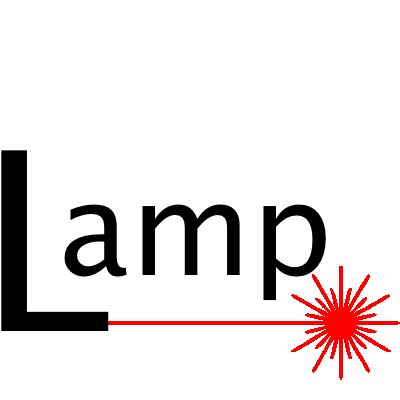
\includegraphics[width=2cm]{lamp.png}
}
\pagestyle{fancy}


\newenvironment{qanda}{\setlength{\parindent}{0pt}}{\bigskip}
\newcommand{\Q}{\bigskip\bfseries Q: }
\newcommand{\A}{\par\textbf{A:} \normalfont}

\let\origdoublepage\cleardoublepage
\newcommand{\clearemptydoublepage}{%
	\clearpage
	{\pagestyle{empty}\origdoublepage}%
}



\begin{document}

	\begin{titlepage}
	\makeatletter
		\centering
		\vfill
		\vfill
		\vfill
		\vfill
		\vfill
		{\bfseries\Huge
				\@title \\
		}
			
			\vfill{
			\bfseries\huge \@author \\ \normalfont\huge Max Wharton-Jones, Shourov Quazi, Jack Jiang
		}
	\vfill{
			\huge{\@date}}

	
		
		\vfill
		\fbox{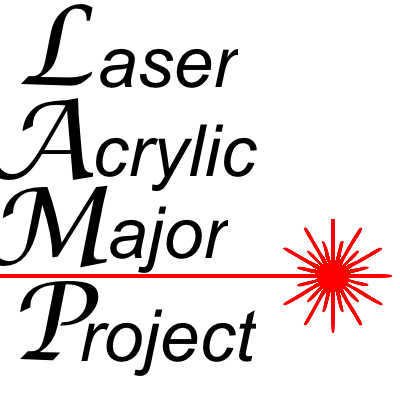
\includegraphics[width=12cm]{title.png} }% also works with logo.pdf
		\vfill
		\vfill
		
			\makeatother
	\end{titlepage}

	\pagenumbering{gobble}
	
	\newpage
	\tableofcontents
	
	
	\pagenumbering{arabic}

	

\chapter{Defining the Problem}
\section[Client Details]{Client Details\protect\footnote{Client Details by Jack}}
\subsection{Clients}
Sydney Boys High School is an academically selective high school conducted by the NSW Department of Education.
The school is led by the senior executive team, comprising the Principal, Dr Kim Jaggar, and Deputy Principals Ms Rachel Powell and Mr Robert Dowdell. The executive staff of nine Head Teachers and the twelve School Administration Officers led by Senior Administrative Manager Ms Sharon Kearns, support the senior executive. The school has three main offices - in the Main Building, in the Ken Andrews Library and in McDonald Wing. Finance, purchasing, enrolment and general inquiries are handled in the main building. Secretarial and network services are the responsibility of the McDonald Wing office.
The clients for this project will be Ms Dam, Mr Comben and Dr Jaggar. Ms Dam and Mr Comben moderate the use of the laser cutter machine and are both teachers in the Industrial Arts department with Ms Dam being the head teacher. They are seeking a better system regarding the use of the laser cutter, especially with cutting trophies for their respective sports. Dr Jaggar is the principal of SBHS, who will be financing the project. Additional users include all other staff at SBHS and all current students of SBHS, however only Staff that are MIC of sports and other extracurricular activities will have access to the creation of trophies. Other staff and students will have access to the template creator only.
\subsection{Current System}
In the current system, all laser cutting requests are handled by the IA staff over email or in person. Individuals send their design files into to the IA staff or go in person to cut their objects with supervision. Only limited number of students and teachers have access to the system, and each job must be signed off by someone from the IA staff. 
Before laser cutting, the file must be checked manually by staff to ensure for correctness, and an often trial-and-error approach is used to ensure the correct settings are applied to each line type. Material is then aligned in the laser cutter, and the piece is cut, a process that can take between 5 minutes to several hours, depending on the complexity and size of the job. Only one job can be cut at once. There is no tracking of jobs, relying on email and paper to track jobs in progress and in queue. Currently, they use a program to help generate one type of template, the school trophy, although this program lacks several features, explored in the interview.
\section[Client Needs Research]{Client Needs Research\protect\footnote{Interview by Shourov}}
\subsection{Interview}
\subsubsection{\textit{Interview with Mr Comben (MIC, IA Teacher)}}
\begin{qanda}
\Q How many physical Awards are given out each year
\A The number varies through the years, but for rifle shooting in particular, there are mainly perpetual awards. For these, we would be looking for brass laser cut plaques.

\Q How much area in the budget is there for extra trophies?
\A Keeping in mind of the cost factor, including the cost for a teacher to operate the laser cutter, as well as the material, there is most likely not that much money available for many of the sports. I know rifle shooting has no area in the budget for extra trophies.

\Q How can we make the laser cutting process more efficient?
\A Look for vector-based fonts, this would allow faster cutting. You want faster cutting speeds to minimise the time spent waiting at the cutter. Also, try to make a reference-based system, this way the amount of time spent setting up the cutting process.

\Q What would be some improvements from the previous system that you would recommend?
\A The old system was very good, although due to the time constraint had many flaws. I would recommend an easier GUI. The old GUI was hard to navigate, and I believe there were some areas that were not functional. Also, the system of setting up the laser cutter took up a large bulk of time. If you can find a way to align the cutter easier, that would be good. Also, the workflow from AutoCAD is very unreliable, I would recommend exporting in illustrator

\Q What were some advantages in terms of resources from the previous system?
\A I can’t say for sure about the budgetary resources saved, but I can say for sure that in the long term, the money saved would easily pay off the laser cutter. Also, the program has inspired a great deal of the industrial tech classes, we now have year 8’s playing around with the potential of the cutter which is great.

\Q Do you have anything you want to see from our program?
\A I would like to see a function that would allow the user to nominate a folder of files that are ready to laser cut, and give the user detailed feedback on the user. Such as, this user has 90\% black line in his work, and would take a long time to finish. This would allow us to check the jobs, and let it be easier to pass works.
\end{qanda}

\subsubsection{\textit{Interview with Ms Dam. (MIC, Supervisor, Head of Industrial Arts)}}
\begin{qanda}
\Q What are the costings of using the laser cutter in reference to the program used last year to create the trophies?
\A Last year, the trophies printed was a great success, especially considering the fact that it was the first year to use the laser cutter. The cost was of course the cost of the trophies from its original source. The profit came from the comparison of the cost of a teacher to be printing and the cost of printing the trophies elsewhere. The cost of a teacher is around \$400 a day whereas each trophy would cost \$10 elsewhere. Hence, if we could print 40 trophies a day, we would be making a profit, which we easily reached.

\Q What would you want to see from our program?
\A From your program I’d like to see it be a lot less time consuming. I would like to spend less time setting up the cutter and more time watching it cut. This would be done as Mr Comben said, to use a reference point system. Also, I would like to see a cleaner GUI.
\end{qanda}

\subsubsection{Needs}

\begin{longtable}{|p{4cm}|p{10cm}|}
	
   \hline
   \rowcolor{gray!50}
   \textbf{Needs} & \textbf{Objectives} \\ \hline
   
   Must store $>50$ different records & 
	\begin{itemize}
		\itemsep0em
   	\item Store $>50$ different templates in a database
	\item Store $>50$ users, clients 
	\item Store fonts and different shapes 
	
	\end{itemize} \\ \hline

	
	
	An editor to create templates & A drag and drop interface supporting
	\begin{itemize}
		\itemsep0em
		\item text with different fonts
		\item circles
		\item rectangles
		\item lines
	\end{itemize} \\ \hline

	
	Use a variety of different materials & Program must indicate the material and settings to use on the laser cutter OR setting these values automatically before a job. \\ \hline
	
	Be cost effective (manpower, trophy cost) & The program must be efficient in the usage and process of its materials. For example, when engraving school trophies for Sydney Boys High School.\newline

	Assuming that: 
	\begin{itemize}
		\itemsep0em
		\item Each trophy laser cut saves \$10
		\item A working day is 5 hours long.
		\item The cost of a Teacher is \$400 a day
	\end{itemize} 
	Then, the program must be optimised such at LEAST 8 trophies can be cut per hour.\\ \hline
	
	
  Minimum Manual work to save time &  Program must assist the user in aligning the job in the laser cutter. Previously this was done manually with callipers. \\ \hline
  
    Improvement on printing capabilities of the last product & To increase efficiency of the cutter: 
  \begin{itemize}
  	\itemsep0em
  	\item Reduce Raster lines
  	\item Increase Vector Lines
  	\item No double lines
  	\item Vector-based fonts
  \end{itemize} \\ \hline


  Improved GUI usability & Current GUI has many issues, that must be rectified in the solution
\begin{itemize}
	\itemsep0em
	\item Hard to navigate
	\item Limited Usage
	\item No tutorial
	\item Some functions don't work like keybindings
	\item Hard to line up
\end{itemize} 
	\begin{center} 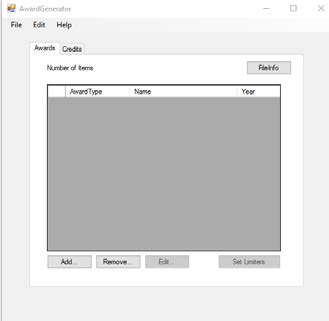
\includegraphics[width=4cm]{examplegui.png}
	\end{center}

 \\ \hline
 
  Export/Import to Illustrator and Autocad & Ability to export/import files compatible with illustrator Illustrator
  AND/OR AutoCAD or other popular cad programs
	 \\ \hline
	 
	 
	 Check Illustrator files for efficiency & A process that reads in an Illustrator file and
	 \begin{itemize}
	 	\itemsep0em
	 	\item Reads all linetypes in the file
	 	\item Compiles linetypes in numerical data
	 	\item Quantitatively assesses linetype data
	 	\item Provides estimate on print time
	 	\item Displays linetype data in readable format
	 \end{itemize} \\ \hline
 
Ability to search and sort templates  & Ability to attach a number of tags to each template, which can be filtered by the user
	\begin{itemize}
		\itemsep0em
		\item Template name
		\item Template creator
		\item Date created/Approved
		\item Item ID
		\item Template material
		\item Purpose, e.g. athletics, rifle shooting
	\end{itemize} \\ \hline

Different levels of access & 3 levels of access, with each level having all the permissions of the levels below
\begin{itemize}
	\itemsep0em
	\item Student (Lowest): can submit templates to be approved then used by teachers/administrators
	\item Teachers: can also submit jobs to administrators for approval, who run the laser cutter. Can also approve templates.
	\item Administrators: have all permissions, can view all information and approve all jobs/templates, to be cut by the laser cutter.
\end{itemize} \\ \hline

\end{longtable}


\subsubsection{Specifications}
The school computers are mostly Dell ThinkCentre machines, with the following specifications \newline 


\begin{longtable}{|p{6cm}|p{6cm}|}
	\hline
	\rowcolor{gray!25}
	\textbf{CPU} &  Intel® Pentium® CPU G3220 @ 3.00 (GHz) \\ \hline

	\textbf{RAM} &  8192MB (8GB) \\ \hline

\rowcolor{gray!25}
	\textbf{Graphics Adapter} &  Intel® HD Graphics \\ \hline

	\textbf{Operating System} &  Windows 10 Pro \\ \hline
	 
\end{longtable}

Therefore, program requirements should include: \\
\begin{longtable}{|p{4cm}|p{4cm}|p{4cm}|}	
	\hline
	\rowcolor{gray!25}
	& \textbf{Minimum Requirements}  & \textbf{Recommended Requirements} \\ \hline
	
	\rowcolor{gray!25}
	\textbf{CPU} &  Dual Core 2 GHz+ &  Quad Core 3 GHz+ \\ \hline
	
	\rowcolor{white}
	\textbf{RAM} &  512 MB &  4GB \\ \hline
	
	\rowcolor{gray!25}
	\textbf{Operating System (Client)} &  Windows 7 &  Windows 7, 8, 10 \\ \hline
	
	\rowcolor{white}
	\textbf{Dependencies (Client)} &  NET Framework 4.0 &  NET Framework 4.0 \\ \hline
	
	\rowcolor{gray!25}
	\textbf{Operating System (Servier)} &  Windows 7, MacOSX 4.0, Ubuntu 16.04+ &  Windows 7+, Ubuntu 16.04+ \\ \hline
	
	
\end{longtable}

\begin{itemize}
	\itemsep0em
	\item We chose to limit the Client Program to the Windows operating system, all the school computers run windows exclusively. However, the server software must be cross platform, as servers are often run from a variety of OS’s (Linux, windows etc.)
	\item The program should run well on school computers, as they meet both the minimum and recommended requirements.
\end{itemize} 

\section[Feasibility Study]{Feasibility Study \footnote{Feasibility Study by Jack}}
\subsection{Market feasibility}
\begin{wrapfigure}{R}{0.4\textwidth} \centering 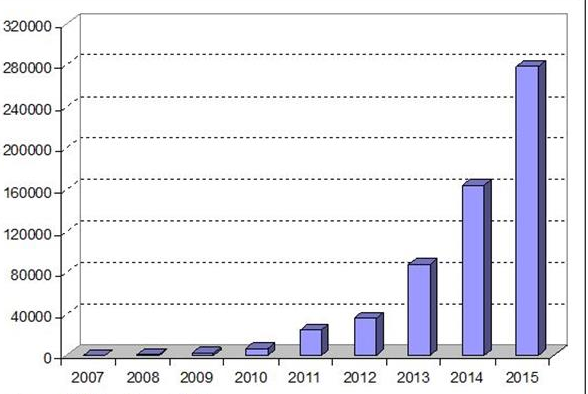
\includegraphics[width=0.4\textwidth]{wrap1.png} \caption{\label{fig:Diagram} Desktop 3D printers sold. Source: Wohlers Report 2016}\end{wrapfigure} 


The proposed plan is to design a software product that will use the laser cutting machine to produce physical products. The project involves several industries: software design, industrial production / manufacturing and product design.

The low volume and DIY (Do it yourself) manufacturing market has flourished, due to the higher availability and the diminishing costs associated with manufacturing. Flexible Manufacturing Systems (FMS), like the laser cutter or 3D printer allow for arbitrary objects to be created from computer-aided designer (CAD) files.

Currently, solutions on the marketplace include: 2D CAD programs, which although work with the laser cutter, becomes inconvenient and inefficient when producing a large quantity of objects with variations, and complex templating solutions which require a significant amount of programming and technical expertise. 
The project involves using a program to aid in the generation and production of files that are sent to the laser cutter. There are few or no off-the-shelf type programs that achieve this, as laser cutting is often a specialised and expensive industrial process. It is often cumbersome for students and teachers to create multiple copies of a single object, which the program seeks to automate
Conclusion:
LAMP focuses on the niche in the market. There are few commercial programs that help with low volume production, a market that has boomed in the last five years. Since the demand for such a software is increasing and there are few competitors, this program will have a well-defined target market, and is market feasible.

\subsection{Technical feasibility}
There are many technical components that need to be researched and experimented on beforehand to ensure that the project's success. Fortunately, the laser cutting project developed last year can be used as a proof of concept, with many technical barriers solved which can be ported over to the new program (existing software).
Designer Technology:
LAMP will include a designer that allows editing of templates dynamically inside the program. It will essentially be a 2D only CAD screen, with options for lines, circles, boxes, shapes and text. Text may be in different sizes and fonts. The designer will allow the three different cutting types to be specified for individual elements (vector cut, vector engrave, raster engrave). This will then be saved in a custom format (.spiff file), which contains all the data required to store the required template. Placeholder elements can be specified in the .spiff file, so that the template can be filled in automatically through the program with a list of names, or years.
\begin{itemize}
	\item Basic 2D CAD interface
	\begin{itemize}
		\itemsep0em
		\item rendering of elements onto screen
		\item optimization to run on lower-powered computers
		\item real dimensions (cm/mm)
		\item zoom
		\item different modes (cutting, engraving)
	\end{itemize}
	
	\item custom file type
	\begin{itemize}
		\itemsep0em
		\item .SPF file contains data on placeholder elements (text that needs to be replaced) and also line/box data
		\item read and write .SPF files
	\end{itemize}
\end{itemize}

\subsection{AutoCAD/Illustrator Interoperability}
The .SPF file will need to be exported to illustrator (.ai) and/or AutocAD (.dxf) files to be used by the laser cutter. The program will also need to be able to take a list of names/years from a document file, using this data to replace the placeholder elements on a template, and layout the template a variable amount of time in the output file in an optimum matter, taking into account the total space in the laser cutter. Manual alignment will also be possible.
\begin{itemize}
	\item export to vector format (ai/dxf)
	\begin{itemize}
		\itemsep0em
        \item writing/reading design files
        \item generating different vector lines
        \item vector fonts
        \item vector lines and curves
    \end{itemize}
    \item read/write document files (.docx, .xlsx, .csv)
    \item layout of multiple copies of template
\end{itemize}

\subsection{Utility and calibration}
The program will have error-checking algorithms on .AI files, to ensure it has lines that are compatible with the laser-cutter. 
\begin{itemize}
	\item read/write illustrator files 
	\begin{itemize}
    	\item file checking algorithm for illustrator files
  	\end{itemize}
\end{itemize}

\subsection{Laser cutter machine}
The laser cutter machine is a complex piece of hardware, capable of cutting thin material via vector lines, and engraving with both vector and raster modes available. The laser bed or cutting space is 450 x 600mm, which will limit the maximum number of trophies cut at once. It uses a 50 watt, 10$\mu$m laser, and the materials it can cut are thin woods and plastics, but it can engrave a variety of materials, including plastics, woods and glass. 
\begin{itemize}
	\itemsep0em
	\item Capabilities of the laser cutter
	\begin{itemize}
		\itemsep0em
    	\item engraves plastics, woods and glass
        \item cuts thin woods and plastics
    \end{itemize}

    	\item Size of the laser cutter (450 x 600mm)
    	\item Safety of operation 

\end{itemize}

\subsection{School Systems}
LAMP stores the approved templates which are available to anyone using the program and the jobs in queue in a server. This may be run locally on the school server, or in a cloud server hosted on SaaS platforms. The files and credentials of users will need to be encrypted, to increase the safety of the system, and some basic measures need to be taken to stop hacking or denial of service (DOS) attempts. This server will come as a separate executable to the client system used by the end user. The client software will need to be able to run on school computers, which mostly have dual-core intel processors with between 8 to 16 gigabytes of ram. Approval from the school’s IT staff may be required to install LAMP’s client software. 
\begin{itemize}
	\item Server Software (if required)
	\begin{itemize}
		\itemsep0em
        \item file and credential encryption
        \item serve requests to list all approved templates
        \item unblocked from school internet 
        \item needs to be secure and reliable
    \end{itemize}
    
    \item Client Software
    \begin{itemize} 
    	\itemsep0em
        \item may need administrator permissions to install on school systems (ask IT).
    	\item will connect to the server through the internet, or the schools internal intranet.
        \item optimization to run on school’s computers
	\end{itemize}
\end{itemize}

\subsubsection{Conclusion}
There are a large number of technical challenges to solve in order for lamp to succeed. Fortunately, several of these have already been addressed in the previous program, and the Industrial Arts staff at school understand the laser cutting system, providing enough information to explain many of the laser-cutting related problems. Over the holidays and throughout the year, research will need to be done on the schools systems, the designer interface and our custom file type. Thanks to the previous program and our teams previous experience with working on the laser cutter, we will be able to focus on these issues instead, reducing the amount of work needed. Overall, the program will be technically feasible. 

\subsection{Financial feasibility}
A middle-end laser cutting machine is an expensive instrument, coming around between \$20,000 - \$100,000. There are cheaper alternatives, but they are slower and/or less precise. However, as the school already has bought a laser cutter, the costs are mostly maintenance and teacher time.
The original trophy system can be used as a proof of concept, and has proven to be cost effective. Expanding this system to other awards may allow for even more cost saving. Awards for different sports account for a significant savings. Costs can be further reduced by bulk buying many trophies from overseas.
Take for example the previous program, which focused on a particular trophy, the School Trophy. Initially it had cost the school 135\$ per trophy, including raw material and engraving costs. However, a blank trophy can be sourced for 15\$, and engraved on the school's cutter. Given that the hourly rate for teachers is 80\$ per hour, with each school trophy taking approximately 15 minutes of time, and producing a trophy in-house would costs 35\$, or a 75\% decrease in cost. LAMP will decrease the time required to setup and cut the trophy, and also allow for other types of trophies to be cut through its templating system, which the old system could not do.

We will require some material and test awards to experiment with the abilities of the laser cutter, which needs to be accounted into our budget. Other costs may include licensing libraries, distribution costs and/or server maintenance. However, even with all these costs factored in, the in-house production of trophies along with other objects will still be cost-effective, saving the school thousands of dollars per annum.

The system will have some server setup and maintenance costs - however, this will be low, as it can be hosted on the school’s existing servers or through inexpensive cloud providers. The program will not need much processing power, and will not handle a large amount of data, further reducing the server costs. Other setup costs include install time and storage space for LAMP’s client software. A developer may be hired to continue to maintain the program after its release, and to fix any bugs discovered after.

LAMP will require a significant amount of developer time, and falling into the medium range in terms of software, probably costing between \$20,000 - \$60,000, based off several other custom software projects. Developer time costs between 75\$ to 200\$ per hour, and the project overall will take around 200-300 hours. The software will be licensed to the school, and may be licensed to multiple schools and businesses. A fee will be charged per user per year, with business subscriptions including priority tech support and user management features. There will be 3 tiers: individual licence will be between 10-30\$ per year for 1 individual, small business (10-1000 users) for 20-40\$ per year per user, and large businesses negotiated separately. Small and large business are also given a copy of the server software that can be setup on their own servers to serve their organisation’s users. This copy will be completely separate from the systems of other businesses, allowing queued jobs and credentials to be kept separately.

\subsubsection{Conclusion}
The project’s main expenses are developer time, and will cost approximately \$40,000. This will be recouped by licensing the software to multiple business and individuals, and charging a yearly fee, which will also help pay the maintenance developers. For the business, LAMP will decrease operational costs by automating parts of the laser cutting process. Therefore, LAMP is financially feasible.

\subsection{Operational feasibility}
\subsubsection{Users}
Users may include teachers and some select students. Teachers will be able to use the program to quickly and easily submit a set of awards for some students. The process should not be changed significantly: the list of students will be sent to the program instead of emailed to an awards seller. The user interface will need to be reliable, consistent and uncomplicated, especially the template designer, which will allow both students and teachers to create the shapes and text without beforehand knowledge of the intricacies of CAD programs and the laser cutter. Little training will be required to use the system for users - pick a template, give some names, submit job. This information will be provided by video tutorials, reference manuals and online help. On-call tech support may be available for business users. Users are able to design templates and/or submit jobs, depending on the permissions given to the user by an administrator.

\subsubsection{Administrators}
Administrators/IA staff will manage and approve request from the users. This will take a significant amount of time, that would otherwise be spent on teaching. To reduce the impact this has, the program will attempt to automate many of the intermediary steps in setting up the laser cutter, and allow for less time calibrating the machine, a process that takes ~10-20 minutes each set of trophies. It will also use more efficient processes to reduce the production time. The program will first be tested on only the industrial arts staff, to ensure the time required to process these trophies will not be an overwhelming amount of work. Administrators have the highest level of access to the program, with permissions to approve both submitted jobs and submitted templates, create and manage users and other administrators, reset passwords etc. This will require a significant amount of training, through video tutorials, reference manuals and online help, with tech support available for businesses. An administrator will require experience with the laser cutter, as they must physically set up the material on the laser cutter in accordance to the current job.
\subsubsection{Conclusion}
For users, the program will require very little training. This means that it will be easy to introduce new users to the system. Administrators will require significant training; however, the industrial arts staff are already accustomed to the laser cutter, easing this process. Support will be given in the form of video tutorials, reference manuals, online support, with on-call technical support for businesses. Overall, this system will not require much training.

\subsection{Social and ethical feasibility}
The program will handle some sensitive data from users - their full name, email, passwords, secret questions and/or contact information will be required by the program in order to operate. This will be stored on the client’s computers, and on LAMP’s server software if applicable. Security will need to be kept in mind to prevent unauthorized access to this sensitive data, through extra security measures taken on the client’s computers, e.g. anti-virus software, correct user privileges, and in the program, e.g. encryption of database, authentication through passwords. Additional server software provides another vector for attackers, and appropriate security measures, like https will need to be used to ensure communications between the program and the server are safe, and to prevent access from unauthorized users. Care will need to be taken to ensure the privacy of the information given to the program by preventing unauthorized access. 
The program should be as inclusive as possible: this would require the program work on lower-powered machines, have an easy and under stable user interface, and users with disabilities considered. Copyright and intellectual property is another possible issue, with appropriate credit given and/or licenses obtained from code included from another source. The program may reduce the amount of time spent laser cutting, but since laser cutting is a secondary job to teaching at Sydney Boys High School, its effect will be negligible on the workforce.
\subsection{Conclusion}
The privacy of users will need to be considered when developing the solution. Appropriate measures need to be taken to prevent unauthorized access. The software should be inclusive to all users, by altering the user interface to suit the needs of individuals.  Intellectual property rights of others need to be considered in the program. 

\subsection{Overall Feasibility}
the issues mentioned with this feasibility study will need to be resolved, but all essential components of the program will be met in the time period set in the Gantt chart

\subsection{Possible Solutions}
Aim: To better use the laser cutting system by simplifying the process required to design and cut objects, and allowing teachers and students limited access into the system.\\


\noindent \textbf{1.  "Upgrade" Approach}

\begin{wrapfigure}{R}{0.3\textwidth} \centering 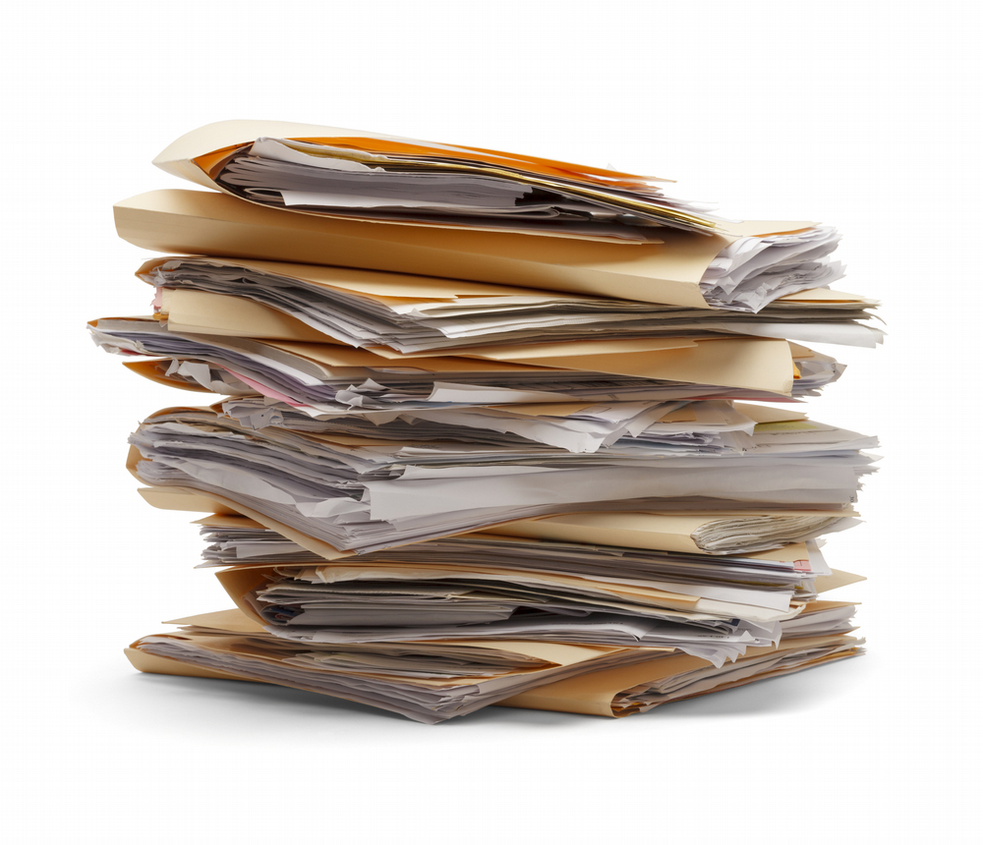
\includegraphics[width=0.3\textwidth]{sol1.png} \end{wrapfigure} 
This approach would see the original trophy generation revisited and revamped to fix issues outlined by staff. In addition, new features could be added, like support for different shapes or awards, and improvements could be made to the GUI to increase its useabilility. This program would only be accessible and usable by IA staff to generate shapes, which can then be rendered by Illustrator a format the laser cutter can use.
	\begin{itemize}
		\itemsep0em
		\item Low cost, complexity and maintance required
		\item Code reuse, which decreases development time and cost
		\item Similar to system already in use, reduceds training required
	\end{itemize} 

\noindent \textbf{2. “Designer” Approach }

\begin{wrapfigure}{R}{0.3\textwidth} \centering 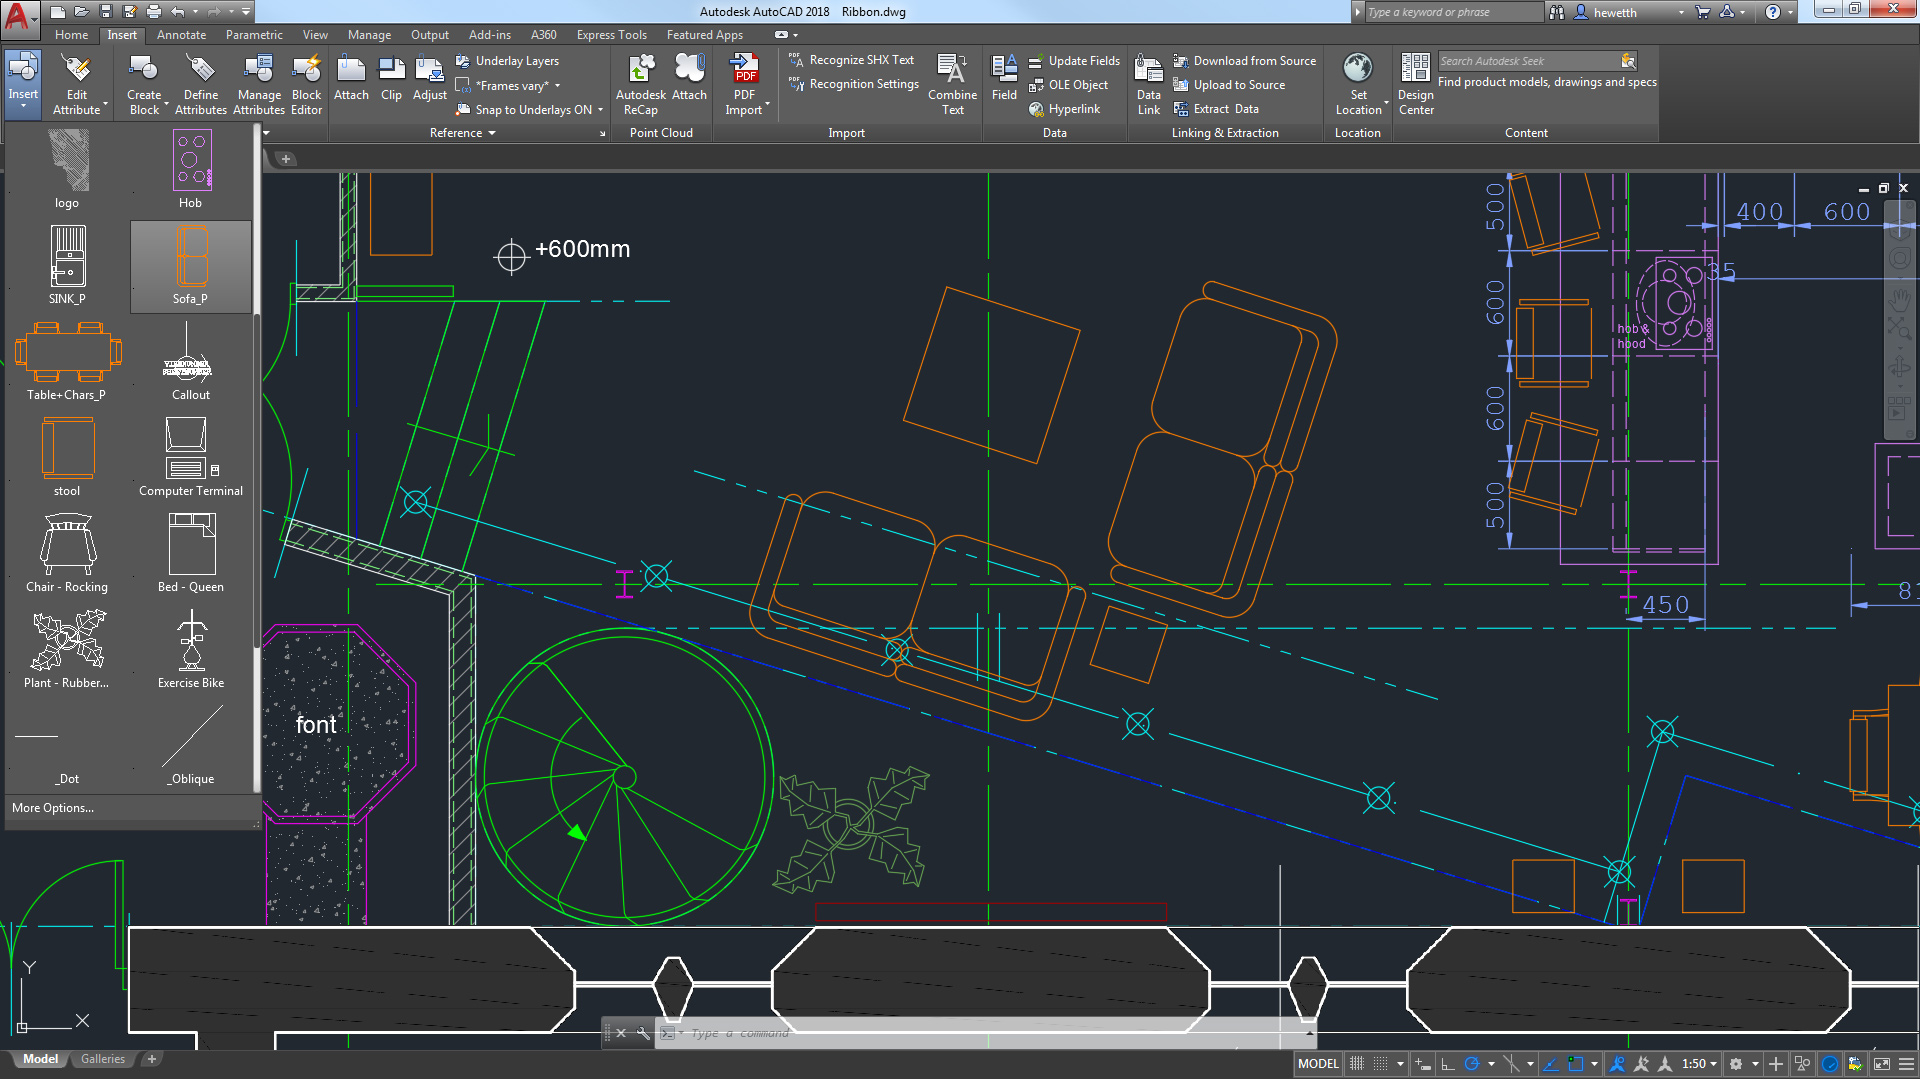
\includegraphics[width=0.3\textwidth]{sol2.png} \end{wrapfigure} 
This approach requires a custom piece of software to be created, and is similar to the system already in use in the school. Using a program to generate a known-good file will allow IA staff to skip several steps in the laser cutting process. However, this incurs additional cost, both in development/setup time and cost. Some basic training and documentation will also need to be provided to the industrial arts teachers using the program. This solution does not attempt to track the created files, relying on email or another form of communication to send and receive files.
	\begin{itemize}
		\itemsep0em
		\item Design tool that loads much faster than AutoCAD and uses less resources
		\item Specialised user interface that contains only the tools required for laser cutting templates
		\item File checking features to ensure linetypes are correct
		\item Automates some printing settings to the laser cutter
	\end{itemize}

\pagebreak
\noindent \textbf{\\ 3. “Server-Client” Approach }

\begin{wrapfigure}{R}{0.3\textwidth} \centering 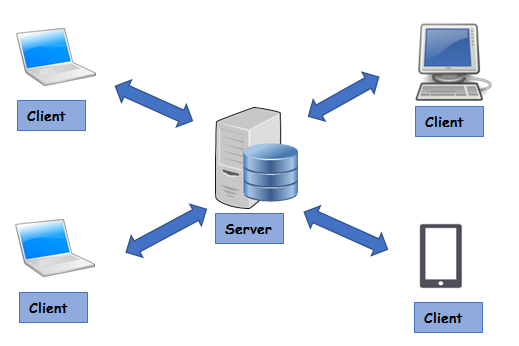
\includegraphics[width=0.3\textwidth]{sol3.png} \end{wrapfigure} 
This approach uses a server to store templates and jobs that users can edit and use. Using a server allows easier communication between the end-users and the IA staff, but incurs additional cost and setup complexity. Using a server also entails an additional, recurring cost of hosting the server. Security over the net could also be an issue, and care will need to be taken to avoid access by unauthorized individuals over the internet. On the other hand, the server-client approach will allow for better tracking of individual jobs, centralization of users to ensure only the correct people have access to the program through user login and server-side checking of files. This system also may allow users/administrators to use the system from multiple places, as long as there is a working internet connection
Features:
	\begin{itemize}
	\itemsep0em
	\item Loads much faster than AutoCAD and uses less resources
    \item Specialised user interface that contains only the tools required for laser cutting templates
    \item File checking features to ensure linetypes are correct
    \item Automates some printing settings to the laser cutter
    \item Templates on server can be accessed from anywhere with an internet connection
    \item Tracking of jobs that are in queue or complete
    \item User and Administrator management
    \end{itemize}


\paragraph{The client has chosen option 3}
The client would like to choose Option 3. Option 1 is far too basic and not really an  the current system. Option 2 again is not an improvement on the current system, as we already use a server. Option 3 contains many new features that could help improve the efficiency of laser cutting, despite the extra cost.

\section[Rights Research]{Rights Research \footnote{Section by Max}}
A software licence determines the use and redistribution of software. It determines how the software can be used by the purchaser of the software, often called the licensee, and may protect the developer legally from damage caused by the software.


\pagebreak 
\textbf{\\There are several types of licences:}\\
\begin{itemize}
	\itemsep0em
	\item Public domain
	\item Open source (FOSS) licenses
	\item Freeware / Shareware
	\item Proprietary
\end{itemize}
 \begin{center}{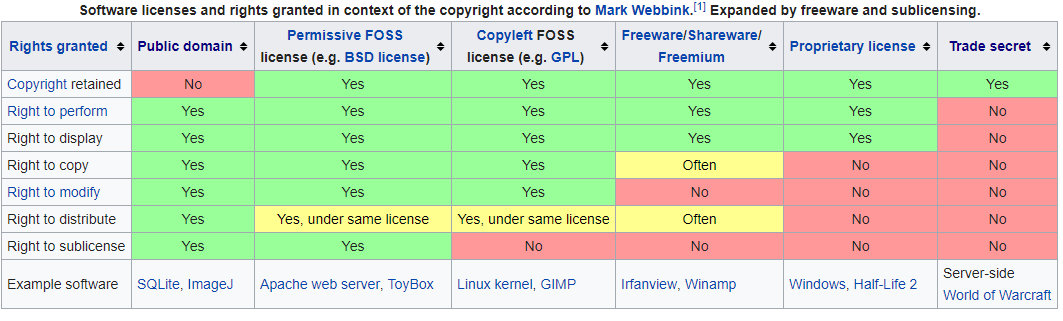
\includegraphics[width=10cm]{licence.png}}
 	\end{center}

Open source licenses, like the GNU GPLv3 licence are for collaborative projects, where developers create code, often for free for their own use.  Any developer can download and alter the source code of a GPL project, but they must provide the altered source code to end-users for their derivative work, display a notice on the program, crediting the original developers of the source code and license their work under the GPL. Many open source projects use this licence, as it ensures that their work will be credited and improvements to the software carried out will be made free to the public. The MIT licence is another software licence. It is a short, simple licence, that allows the alteration of source code with no other conditions. Both these open source licences disclaim any warranties or responsibilities of the original developer in the quality and usability of the code.

\noindent \fbox{
	\parbox{\textwidth}
{Copyright $<$2017-2018$>$ $<$Max Wharton-Jones$>$
	
	Permission is hereby granted, free of charge, to any person obtaining a copy of this software and associated documentation files (the "Software"), to deal in the Software without restriction, including without limitation the rights to use, copy, modify, merge, publish, distribute, sublicense, and/or sell copies of the Software, and to permit persons to whom the Software is furnished to do so, subject to the following conditions:
	The above copyright notice and this permission notice shall be included in all copies or substantial portions of the Software.
	THE SOFTWARE IS PROVIDED "AS IS", WITHOUT WARRANTY OF ANY KIND, EXPRESS OR IMPLIED, INCLUDING BUT NOT LIMITED TO THE WARRANTIES OF MERCHANTABILITY, FITNESS FOR A PARTICULAR PURPOSE AND NONINFRINGEMENT. IN NO EVENT SHALL THE AUTHORS OR COPYRIGHT HOLDERS BE LIABLE FOR ANY CLAIM, DAMAGES OR OTHER LIABILITY, WHETHER IN AN ACTION OF CONTRACT, TORT OR OTHERWISE, ARISING FROM, OUT OF OR IN CONNECTION WITH THE SOFTWARE OR THE USE OR OTHER DEALINGS IN THE SOFTWARE.
	\begin{center}\textbf{The MIT Licence}
		\end{center}
}
}

Freeware licences may use ads or donations in order to make a profit. However, it often lacks enterprise support. Shareware uses locked features or a trial period, allowing users to try out the software before committing to a purchase. 

Open source licences are unsuitable for our project, as they require the distribution of source code. In addition, there is no need for an open source licence as the project will only be created and maintained by our team. A freeware / Shareware licence is unsuitable, as our program will mostly target large organisations, who are willing to pay extra in return for support. Therefore, the proprietary licence will be the most suitable. The software will be maintained by our team, allowing for more features and bug fixes when discovered, funded by the licensing fee. The safety, reliability and usability of the program is essential, as it involves the laser cutter, an expensive and potentially dangerous machine. 
\subsection{IP rights}
Waxy LASER Solutions retains all intellectual property rights to the software. This is necessary so that the program can be licensed to other businesses, and to allow the program to be maintained by our team in the future. 


\subsection{Contract}
\centering\Large\textbf{L.A.M.P - Terms and conditions - Waxy LASER Solutions}\\
\rule{\textwidth}{2pt}

\flushleft
\small
\noindent 1. \textbf{Preamble:} This Agreement, signed on Dec 6, 2017 (hereinafter: Effective Date) governs the relationship between Sydney Boys High School, a School Entity, (hereinafter: Licensee) and L.A.M.P, a partnership under the laws of whose principal place of School is 556 Cleveland St, Moore Park NSW 2021 (hereinafter: Licensor). This Agreement sets the terms, rights, restrictions and obligations on using L.A.M.P (hereinafter: The Software) created and owned by Licensor, as detailed herein

\noindent\rule{\textwidth}{0.5pt}
\noindent 2. \textbf{License Grant:} Licensor hereby grants Licensee a Personal, non-assignable and non-transferable, commercial, royalty free, non-exclusive license, all with accordance with the terms set forth and other legal restrictions set forth in 3rd party software used while running Software.


\begin{enumerate}
	\item Limited: Licensee may use Software for the purpose of: \begin{enumerate}
		\item Running Software on Licensee’s Website[s] and Server[s]; 
		\item Allowing 3rd Parties to run Software on Licensee’s Website[s] and Server[s]; 
		\item Publishing Software output to Licensee and 3rd Parties; 
		\item Distribute verbatim copies of Software’s output (including compiled binaries);
	\end{enumerate}
\item This license is granted perpetually, as long as it is not materially breached.
\item \textbf{Binary Restricted:} Licensee may sublicense Software as a part of a larger work containing more than Software, distributed solely in Object or Binary form under a personal, non-sublicensable, limited license. Such redistribution shall be limited to 1600 codebases.
\item \textbf{Non-Assignable and Non-Transferable:} Licensee may not assign or transfer his rights and duties under this license.
\item \textbf{Commercial, Royalty Free:} Licensee may use Software for any purpose, including paid-services, without any royalties

\end{enumerate}

\noindent\rule{\textwidth}{0.5pt}
\noindent 3. \textbf{Term \& Termination:} The Term of this license shall be until terminated. Licensor may terminate this Agreement, including Licensee’s license in the case where Licensee:
\begin{enumerate}
	\item became insolvent or otherwise entered into any liquidation process; or
\item exported The Software to any jurisdiction where licensor may not enforce his rights under this agreements in; or
\item Licensee was in breach of any of this license's terms and conditions and such breach was not cured, immediately upon notification; or
\item Licensee in breach of any of the terms of clause 2 to this license; or
\item Licensee otherwise entered into any arrangement which caused Licensor to be unable to enforce his rights under this License.
\end{enumerate}

\noindent\rule{\textwidth}{0.5pt}
\noindent 4. \textbf{Payment:} In consideration of the License granted under clause 2, Licensee shall pay Licensor a fee, via Credit-Card, PayPal or any other mean which Licensor may deem adequate. Failure to perform payment shall construe as material breach of this Agreement.

\noindent\rule{\textwidth}{0.5pt}
\noindent 5. \textbf{Upgrades, Updates and Fixes:} Licensor may provide Licensee, from time to time, with Upgrades, Updates or Fixes, as detailed herein and according to his sole discretion. Licensee hereby warrants to keep The Software up-to-date and install all relevant updates and fixes, and may, at his sole discretion, purchase upgrades, according to the rates set by Licensor. Licensor shall provide any update or Fix free of charge; however, nothing in this Agreement shall require Licensor to provide Updates or Fixes.
\begin{enumerate} 
	\item Upgrades: for the purpose of this license, an Upgrade shall be a material amendment in The Software, which contains new features and or major performance improvements and shall be marked as a new version number. For example, should Licensee purchase The Software under version 1.X.X, an upgrade shall commence under number 2.0.0.

\item Updates: for the purpose of this license, an update shall be a minor amendment in The Software, which may contain new features or minor improvements and shall be marked as a new sub-version number. For example, should Licensee purchase The Software under version 1.1.X, an upgrade shall commence under number 1.2.0.
\item Fix: for the purpose of this license, a fix shall be a minor amendment in The Software, intended to remove bugs or alter minor features which impair the The Software's functionality. A fix shall be marked as a new sub-sub-version number. For example, should Licensee purchase Software under version 1.1.1, a fix shall commence under number 1.1.2.
\end{enumerate}

\noindent\rule{\textwidth}{0.5pt}
\noindent 6. \textbf{Support:} Software is provided under an AS-IS basis and without any guarantees of updates or maintenance. Nothing in this Agreement shall require Licensor to provide Licensee with fixes to any bug, failure, mis-performance or other defect in The Software.
\begin{enumerate}
	\item Bug Notification: Licensee may provide Licensor of details regarding any bug, defect or failure in The Software promptly and with no delay from such event; Licensee shall comply with Licensor's request for information regarding bugs, defects or failures and furnish him with information, screenshots and try to reproduce such bugs, defects or failures.
\item Feature Request: Licensee may request additional features in Software, provided, however, that 
\begin{enumerate} 
	\item Licensee shall waive any claim or right in such feature should feature be developed by Licensor; 
	\item Licensee shall be prohibited from developing the feature, or disclose such feature request, or feature, to any 3rd party directly competing with Licensor or any 3rd party which may be, following the development of such feature, in direct competition with Licensor; 
	\item Licensee warrants that feature does not infringe any 3rd party patent, trademark, trade-secret or any other intellectual property right; and 
	\item Licensee developed, envisioned or created the feature solely by himself.
\end{enumerate}
\end{enumerate}

\rule{\textwidth}{0.5pt}
\noindent 7. \textbf{Liability:}  To the extent permitted under Law, The Software is provided under an AS-IS basis. Licensor shall never, and without any limit, be liable for any damage, cost, expense or any other payment incurred by Licensee as a result of Software’s actions, failure, bugs and/or any other interaction between The Software and Licensee’s end-equipment, computers, other software or any 3rd party, end-equipment, computer or services.  Moreover, Licensor shall never be liable for any defect in source code written by Licensee when relying on The Software or using The Software’s source code.

\noindent\rule{\textwidth}{0.5pt}
\noindent 8. \textbf{Warranty: }
\begin{enumerate}
	\item Intellectual Property: Licensor hereby warrants that the Software does not violate or infringe any 3rd party claims in regards to intellectual property, patents and/or trademarks and that to the best of its knowledge no legal action has been taken against it for any infringement or violation of any 3rd party intellectual property rights.
\item No-Warranty: The Software is provided without any warranty; Licensor hereby disclaims any warranty that The Software shall be error free, without defects or code which may cause damage to Licensee’s computers or to Licensee, and that Software shall be functional. Licensee shall be solely liable to any damage, defect or loss incurred as a result of operating software and undertake the risks contained in running The Software on Licensee’s Server[s] and Website[s].
\item  Prior Inspection: Licensee hereby states that he inspected The Software thoroughly and found it satisfactory and adequate to his needs, that it does not interfere with his regular operation and that it does meet the standards and scope of his computer systems and architecture. Licensee found that The Software interacts with his development, website and server environment and that it does not infringe any of End User License Agreement of any software Licensee may use in performing his services. Licensee hereby waives any claims regarding The Software's incompatibility, performance, results and features, and warrants that he inspected the The Software.
\end{enumerate}

\noindent\rule{\textwidth}{0.5pt}
\noindent 9. \textbf{No Refunds:} Licensee warrants that he inspected The Software according to clause 7 and that it is adequate to his needs. Accordingly, as The Software is intangible goods, Licensee shall not be, ever, entitled to any refund, rebate, compensation or restitution for any reason whatsoever, even if The Software contains material flaws.

\noindent\rule{\textwidth}{0.5pt}
\noindent 10. \textbf{Indemnification:} Licensee hereby warrants to hold Licensor harmless and indemnify Licensor for any lawsuit brought against it in regards to Licensee’s use of The Software in means that violate, breach or otherwise circumvent this license, Licensor's intellectual property rights or Licensor's title in The Software. Licensor shall promptly notify Licensee in case of such legal action and request Licensee’s consent prior to any settlement in relation to such lawsuit or claim.

\noindent\rule{\textwidth}{0.5pt}
\noindent 11. \textbf{Governing Law, Jurisdiction:} Licensee hereby agrees not to initiate class-action lawsuits against Licensor in relation to this license and to compensate Licensor for any legal fees, cost or attorney fees should any claim brought by Licensee against Licensor be denied, in part or in full
\noindent\rule{\textwidth}{0.5pt}

\normalfont

\chapter{Planning and Designing}
\section[Context Data flow diagrams]{Context Diagram and Data flow diagrams \protect\footnote{Context and DFD by Max}}
\centering
	\fbox{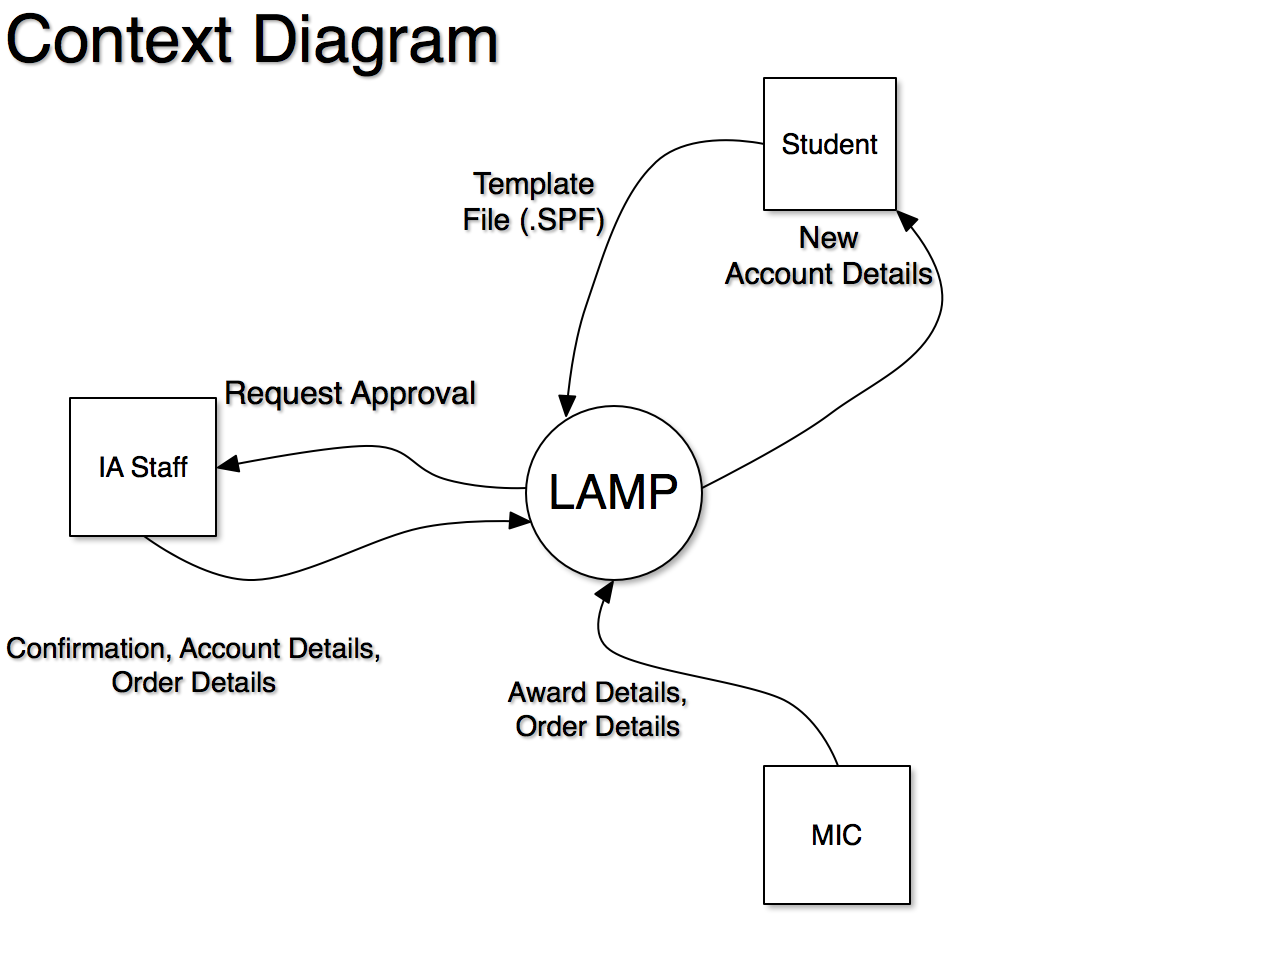
\includegraphics[width=10cm, height=5.5cm]{contextdiagram.png}}

	\fbox{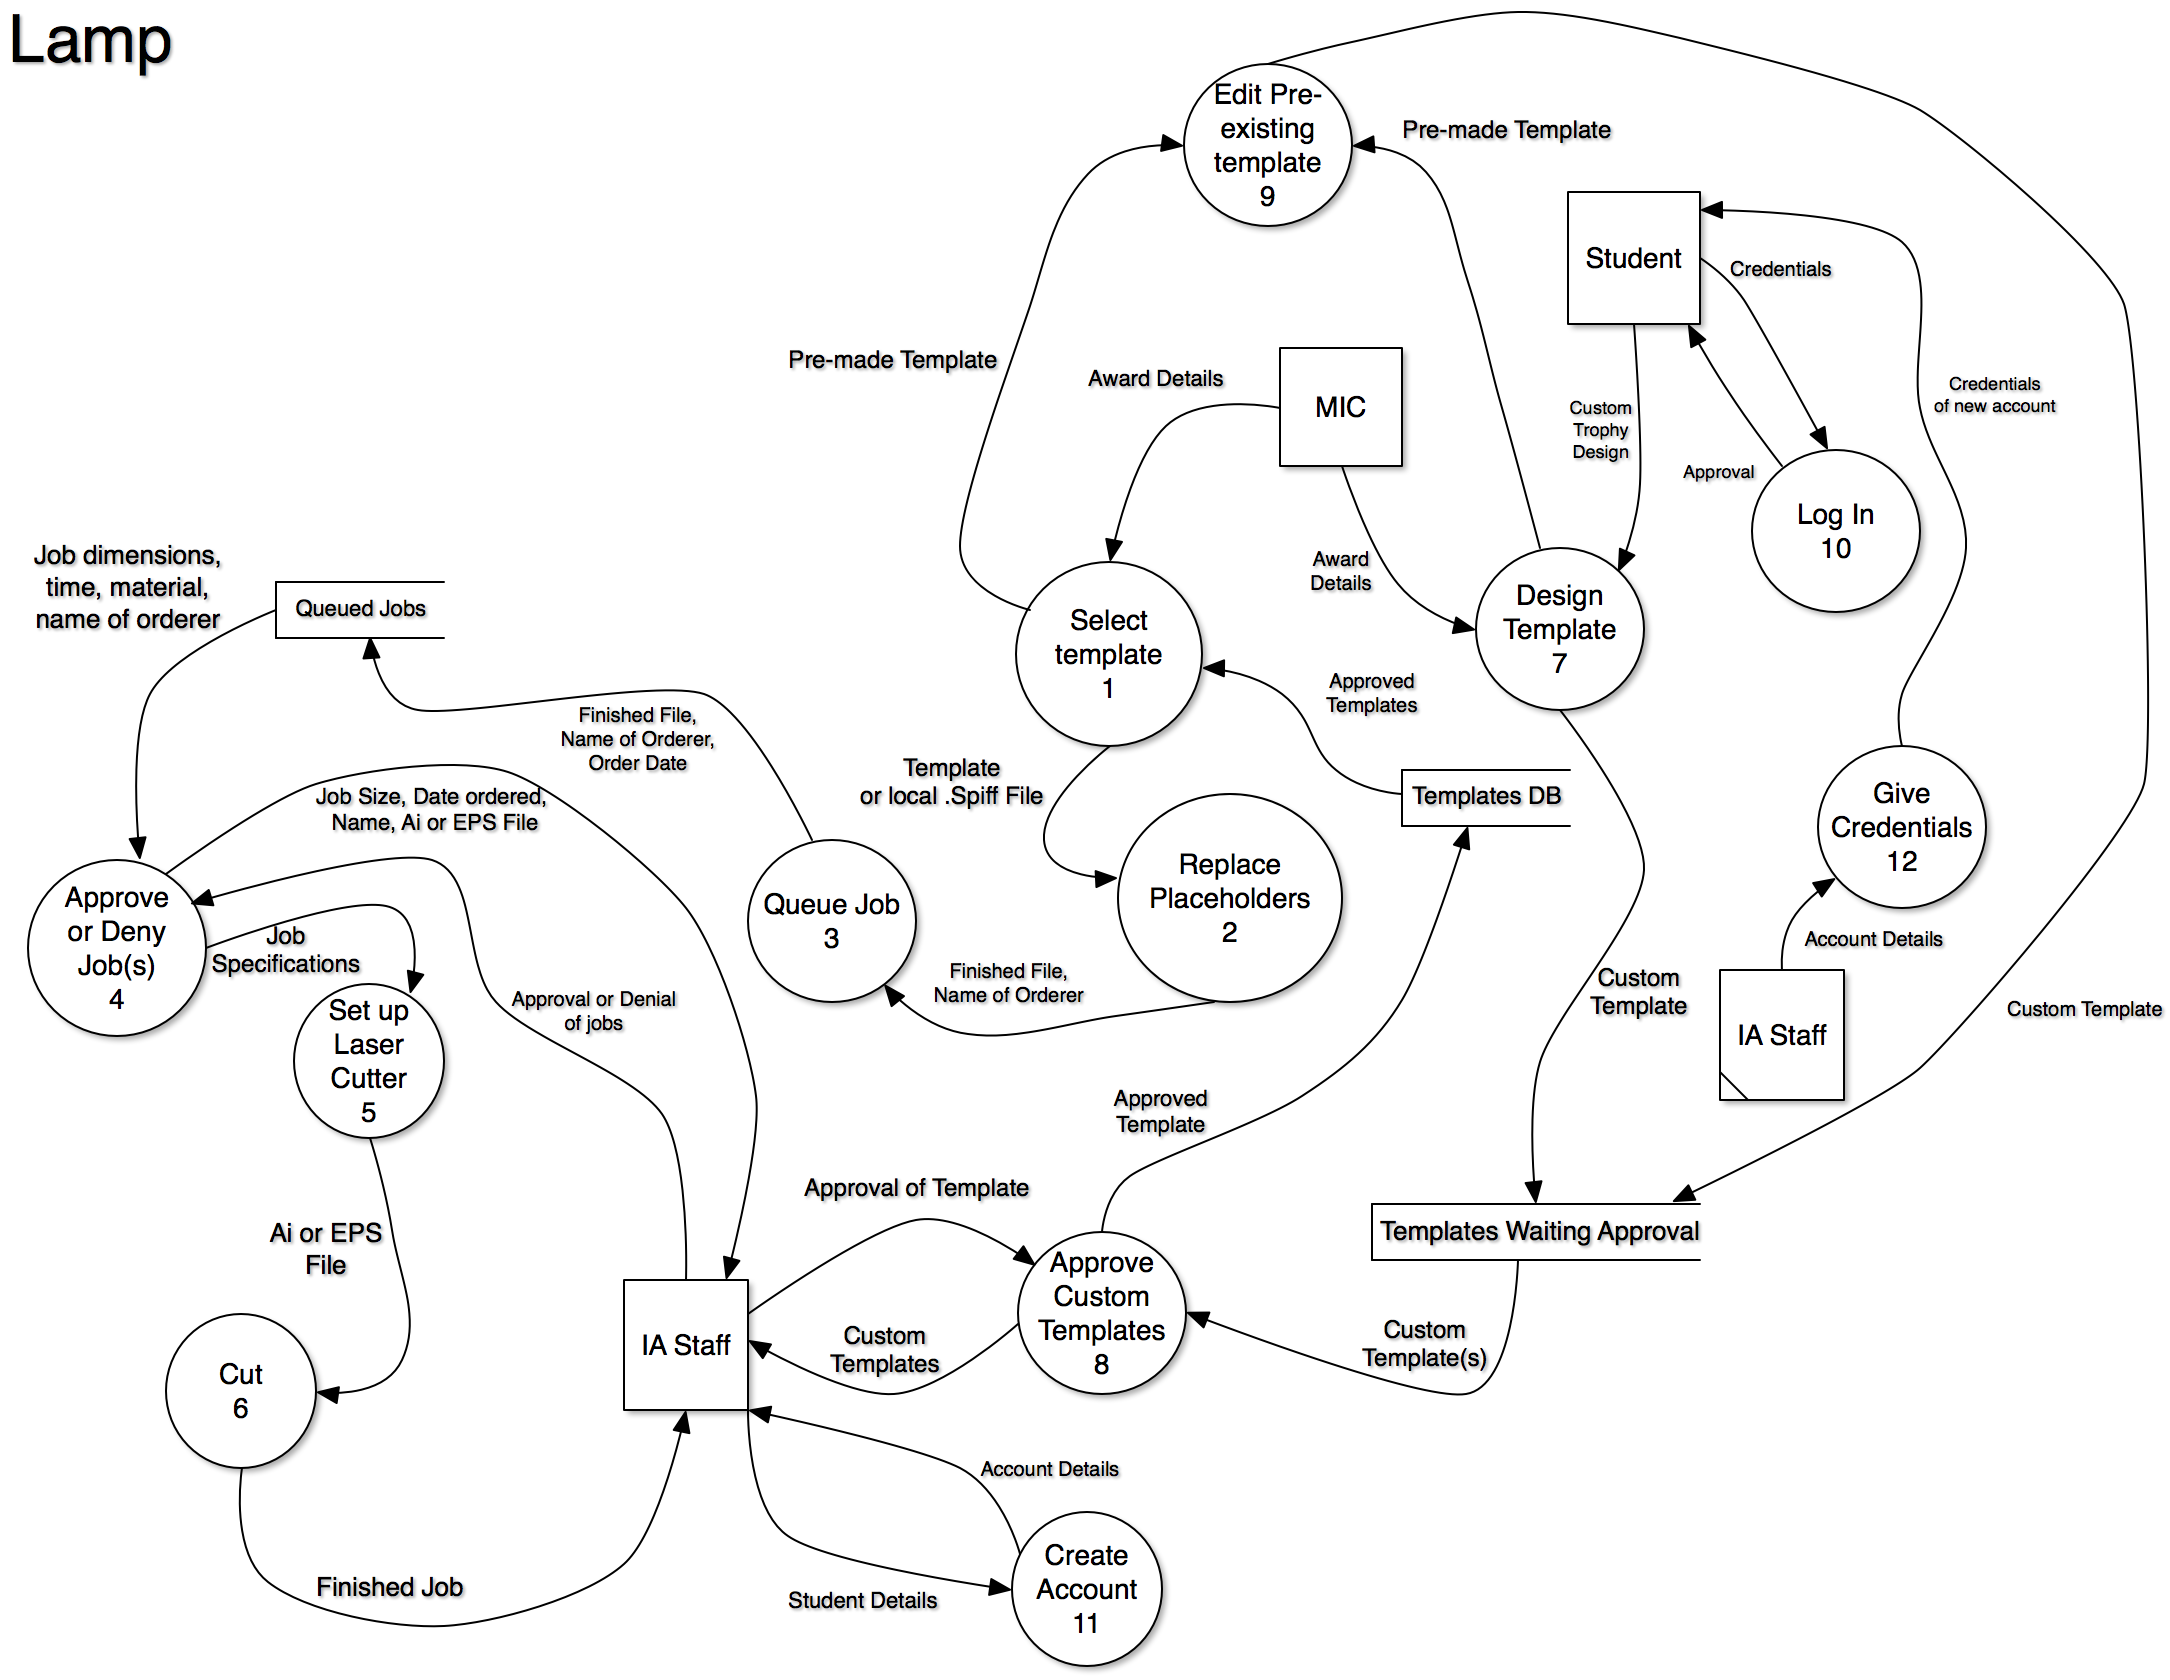
\includegraphics[width=\textwidth, height=7cm]{dfdlvl1.png}}
		\fbox{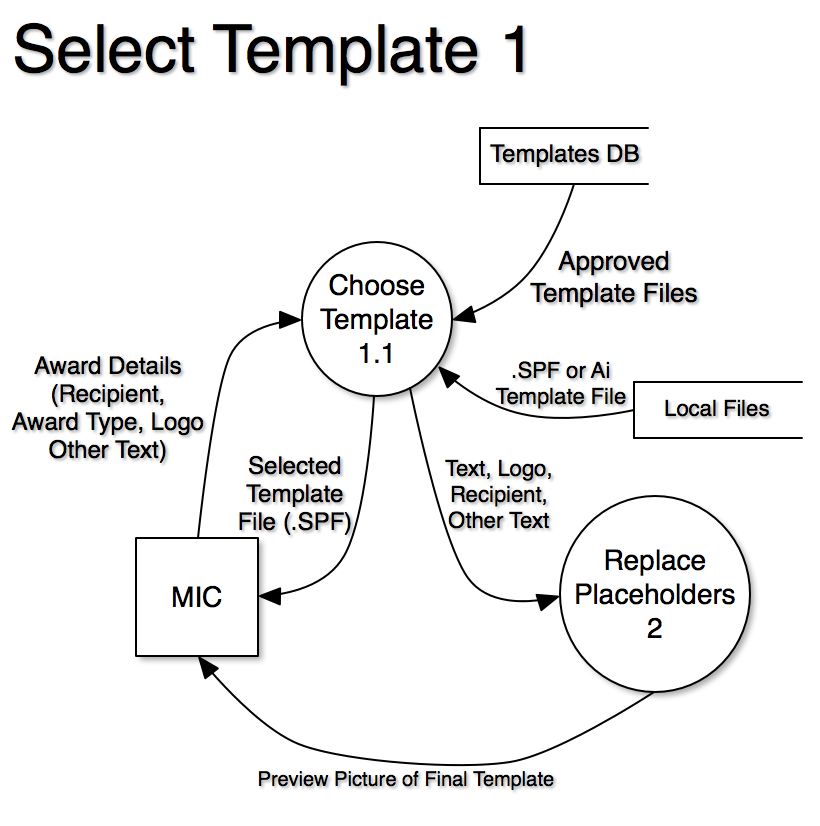
\includegraphics[width=\textwidth, height=10cm]{dfdlvl21.png}}
			\fbox{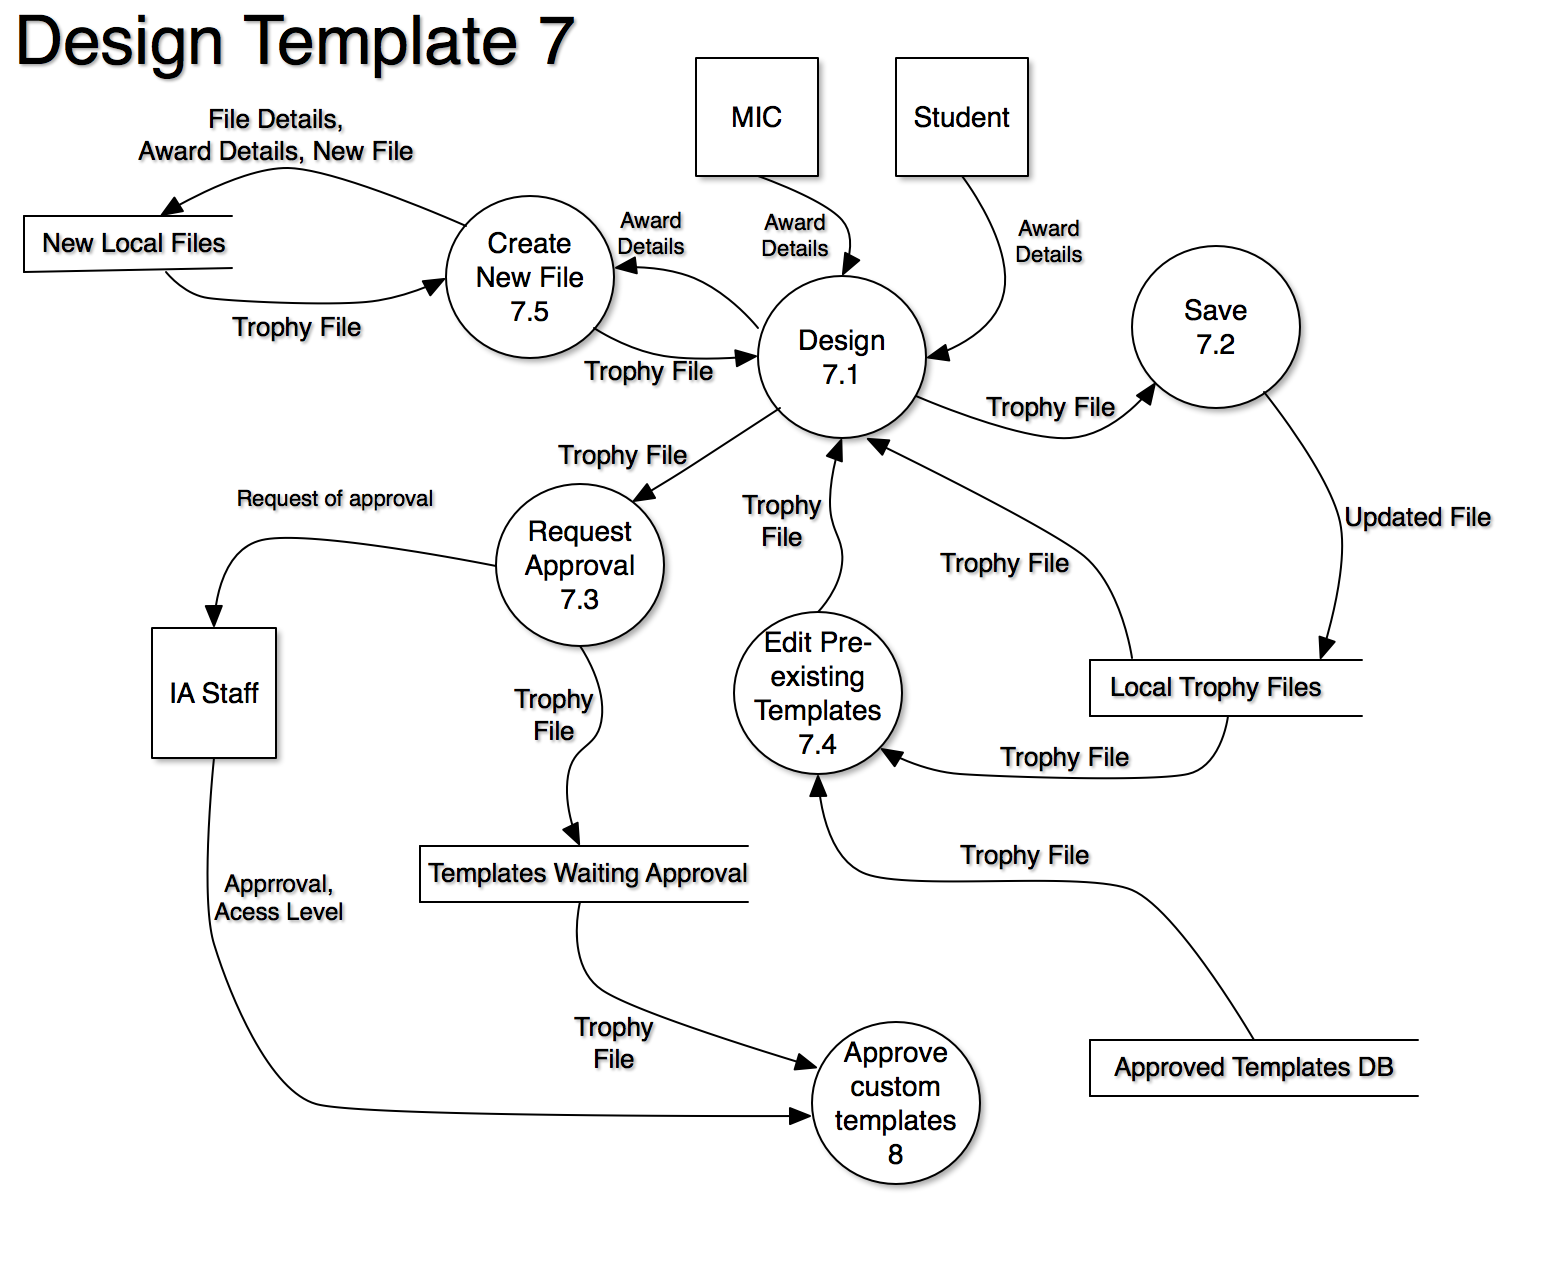
\includegraphics[width=\textwidth, height=10cm]{dfdlvl22.png}}


\section[System Flowchart]{System Flowchart \protect\footnote{System Flowchart By Jack}}
\fbox{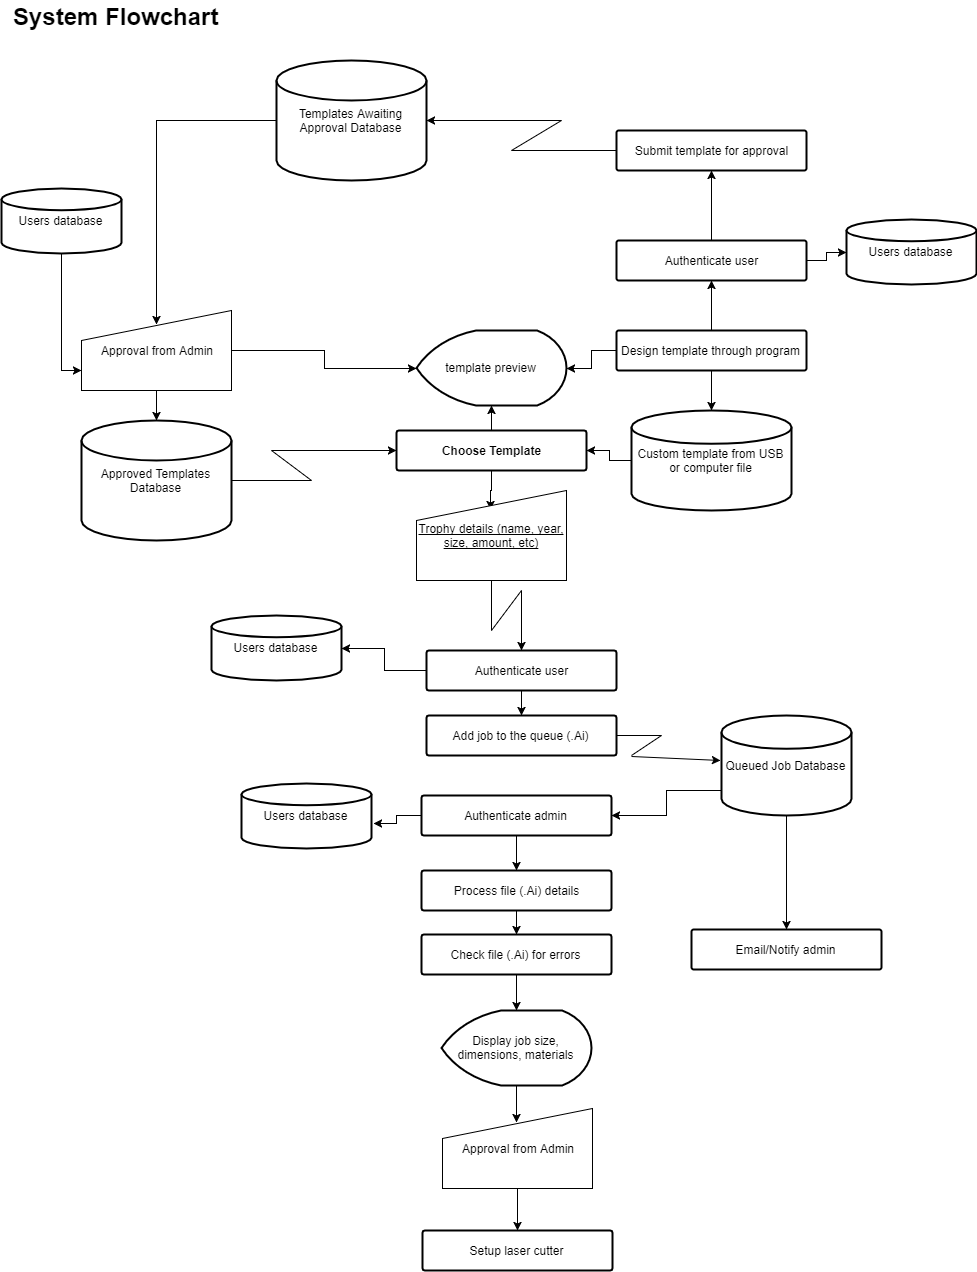
\includegraphics[width=\textwidth]{systemflowchart.png}}

\section[IPO Chart]{IPO Chart \protect\footnote{IPO Chart by Shourov}}
\centering
\subsection{Select Template}
\begin{longtable}{|p{3cm}|p{5cm}|p{4cm}|}	
	\hline
	\rowcolor{gray!40}
	\textbf{Input} & \textbf{Process}  & \textbf{Output} \\ \hline
	
	\rowcolor{white}
	\textbf{Array of SPF files} &  
	Obtains Template From Database \newline
	Displays all template designs in the template database \newline
	Client selects appropriate template from the database
	 &  Partial SPF File containing data for the template selected \\ \hline
	
	\rowcolor{gray!25}
	\noindent \textbf{
		Names (string) \newline
		Number of Awards (int) \newline
		Args*(vary)
	} &  Adds Data to the SPF file containing the type of template already chosen \newline
* \textit{based on the template chosen, the user will be prompted for certain data. An example is for a trophy that requires both a name and a score. The user will be prompted to enter the name as well as the score. If left blank, the input will be considered invalid unless otherwise specified.}
 &  Complete SPF File containing both the selected template data as well as the variation data specified by the user \\ \hline
	
\end{longtable}

\subsection{Design Template}
\begin{longtable}{|p{3cm}|p{5cm}|p{4cm}|}	
	\hline
	\rowcolor{gray!40}
	\textbf{Input} & \textbf{Process}  & \textbf{Output} \\ \hline
	
	\rowcolor{white}
	\textbf{Array of SPF files} &  
	Creates Template from Selection \newline
	Selection From Client  \newline
	\begin{itemize}
		\itemsep0em
		\item Presented as a selection GUI
		\item Displays all template designs in the template data base
		\item Client selects appropriate template from the database
  \end{itemize}
	&  Partial SPF File containing data for the template selected \\ \hline
	
	
	
	\rowcolor{gray!25}
	\noindent \textbf{
		Raw AI / EPS Template File
	} &  Edits Template with Graphical Editor \newline
Graphical Editor
\begin{itemize}
	\itemsep0em
	\item Editor Based off of CAD software
	\item Tools include Line creation
	\item Ability to add images
	\item Ability to add dynamic text \footnotemark
	\item Ability to add static text \footnotemark
	\item Ability to create CUT lines and ENGRAVE lines
\end{itemize}
	&  AI / EPS Template File\\ \hline
	
	\rowcolor{white}
	\textbf{Login / Password (string)} &  
	Authenticates User
	&  Authentication Level (Admin / Teacher / Student) \\ \hline
	
	\rowcolor{gray!25}
	\textbf{AI / EPS Template File \newline
		Authentication level of Client(integer)} &  
	Sends to get verified
	& None \\ \hline
	
	
	
\end{longtable}
\footnotetext[4]{Dynamic text is text which is different for each job from the template file. An example of Dynamic text is the name on a trophy
}
\footnotetext[5]{Static text is text which appears on every job from the template file. An example of Static text is the year on a trophy}

\subsection{Queue Job}
\begin{longtable}{|p{5cm}|p{3cm}|p{4cm}|}	
	\hline
	\rowcolor{gray!40}
	\textbf{Input} & \textbf{Process}  & \textbf{Output} \\ \hline
	
	\rowcolor{white}
	\textbf{Login / Password (String)} &  
	Authentication
	&  Authentication Level (Admin / Teacher / Student) \\ \hline
	
		\rowcolor{gray!25}
	\textbf{SPF File containing \begin{itemize}
			\itemsep0em
			\item Template Selected from Template Database
			\item Variation Data unique to the job required to client
			\item Authentication level of Client
			\item Client Details
		\end{itemize}
	} &  
	Add to Job Queue Database
	& Reponse code \\ \hline
	\end{longtable}

\subsection{Approve Job}
\begin{longtable}{|p{3cm}|p{5cm}|p{4cm}|}	
	\hline
	\rowcolor{gray!40}
	\textbf{Input} & \textbf{Process}  & \textbf{Output} \\ \hline
	
	\rowcolor{white}
	\textbf{Login / Password (String)} &  
	Authentication
	&  IF Authentication level is not Admin deny Approval ability \\ \hline
	
	\rowcolor{gray!25}
	\textbf{SPF File from Job Queue DB} &  
	Approval Process \newline
	Admin level client will see
	\begin{itemize}
		\itemsep0em
		\item Preview of SPF File
		\item Line weight detail of the SPF file
		\item Authentication level of the user
		\item Client Details
	\end{itemize}
	& IF Approved the job is sent to a folder to be laser cut \newline 
	The SPF File is converted to AI / EPS files to match the format of the Laser Cutter. If required, the job is split into multiple files \newline
	IF Not Approved the job is deleted
	\\ \hline
\end{longtable}


\subsection{Set Up Laser Cutter}
\begin{longtable}{|p{3cm}|p{5cm}|p{4cm}|}	
	\hline
	\rowcolor{gray!40}
	\textbf{Input} & \textbf{Process}  & \textbf{Output} \\ \hline
	
	\rowcolor{white}
	\textbf{Login / Password (String)} &  
	Authentication
	&  IF Authentication level is not Admin deny Approval ability \\ \hline
	
	\rowcolor{gray!25}
	\textbf{AI / EPS File} &  
	Laser Cutter Process
	\begin{itemize}
		\itemsep0em
		\item An Admin must place the resource within the Laser Cutter
		\item Open the files on the Laser Cutter computer
		\item Print via Laser Cutter printer to the Laser Cutter
		\item Remain by the Laser Cutter until the job is finished
		\item Remove finished job and replace material if need be
	\end{itemize}
	& Final Job

	\\ \hline
\end{longtable}

\section[Gantt Chart]{Gantt Chart \protect\footnote{Gantt Chart by Shourov}}
\begin{figure}[!htb]
	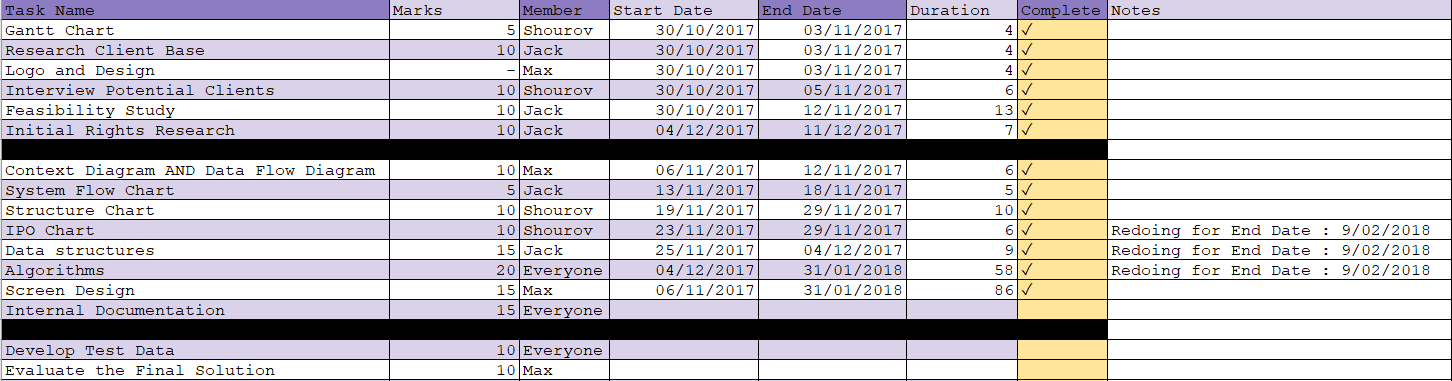
\includegraphics[width=\textwidth]{ganttchart1.png}
	\\
	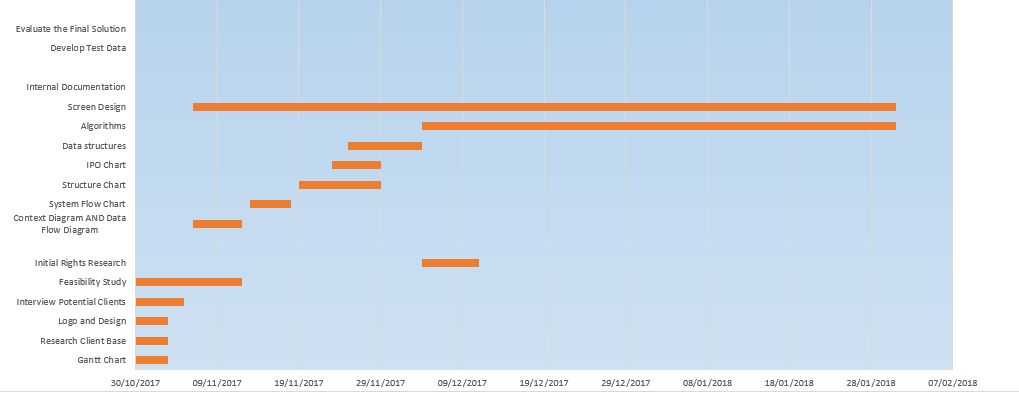
\includegraphics[width=\textwidth]{ganttchart2.png}
\end{figure}


\section[Data Dictionary]{Data Dictionary \protect\footnote{Data Dictionary by Jack}}

\tiny
\begin{longtable}{|p{2cm}|p{3cm}|p{1.5cm}|p{6cm}|}	
	
	\hline
	\rowcolor{gray!25}
	
	\small \textbf{Data Structure} & \small\textbf{Data Type}  & \small\textbf{Length \footnotemark} & \small\textbf{Description} \\ \hline
	

		\multirow{16}{*}{\parbox{2cm}{tblTemplates Array  (TemplateRecord)} }
		& Array(Of Record) &   &  Contains details about approved templates created using the program. can be saved/loaded as .SPF files \\ 
		
		& Auto\textunderscore ID (Auto Number) & 32 & Index 0-2147,483,647 (for database). Primary Key  \\
		& DXF  (String) & 10000 & Line and text data encoded using the DXF format \\
		& tags (Array(Of String)) & 20x20 & the criteria that the template meets \\
		& material (String) & 10 & the material that the template uses\\
		& length (real) & 8 & the length of each piece, in millimeters\\
		& height (real) & 8 & the height of each piece, in millimeters\\
		& thickness (real) & 8 & the thickness of each piece, in millimeters \\
		& preview (Array(Of Image)) & 3x4MB & preview images for each template \\
		& creatorId (Integer) & 4 & id of the creator, joined to tblUser.Auto\textunderscore ID\\
		& approverId (Integer) & 4 & id of the approver, joined to tblUser.Auto\textunderscore ID \\
		& dynamicTextList(Array(Of String)) & 10x10 & Dynamic texts are text labels that are filled in by the user. They describe the name of the label (e.g. year) \\
		& textLocation(Array(Of Point)) & 10x16 & the location where the dynamic text will be filled \\ \hline
		
			\multirow{7}{*}{\parbox{2cm}{tblSumittedJobs Array  (JobRecord)} }
		& Array(Of Record) &   &  Contains information about jobs submitted to the IA staff for cutting.  \\ 
		
		& Auto\textunderscore ID (Auto Number) & 32 & Index 0-2147,483,647 (for database). Primary Key  \\
		& template\textunderscore ID & 32 & the id of the spf file to cut. Joined to tblTemplates.Auto\textunderscore ID \\
		& submitterId (Integer) & 4 & the id of submitter. Joined to tblUser.\textunderscore ID \\
		& approverId (Integer) & 4 & the id of approver. Joined to tblUser.\textunderscore ID \\
		& approved (boolean) & 1 & whether or not the job is approved \\
		& submitDate (date) & 32 & the date in which the job is submitted\\
		\hline
		
			\multirow{6}{*}{\parbox{2cm}{tblUsers Array (UserRecord)} }
		& Array(Of Record) &   &   Contains information about all the users that are stored in the database \\ 
		
		& Auto\textunderscore ID (Auto Number) & 32 & Index 0-2147,483,647 (for database). Primary Key  \\
		& email (string) & 20 & the email used to sign up \\
		& password (string) & 20 & password used to sign in\\
		& accesslevel (integer) & 4 & 1=student, 2=teacher, 3=admin. Determines if the user can do certain actions \\
		& name (string) & 20 & full name of the user \\
		\hline

		\multirow{8}{*}{\parbox{2cm}{lines Array (newline)}}
		& Array (Of Record) & & Stores data about a shape or line drawn using the template designer. Lines is the array containing all the currently drawn lines \\
		& point1x (real) & 8 &start point x co-ordinate \\
			& point1y (real) & 8 &start point y co-ordinate \\
				& point2x (real) & 8 &end point x co-ordinate \\
					& point2y(real) & 8 &end point y co-ordinate \\
						& lineType (string) & 20 & the type of shape drawn\\
						& color (string) & 20 & color of line\\
						& lineNumber (integer) & 4 & the index of the line in the array\\\hline
		\multirow{3}{*}{\parbox{2cm}{Point}}
		& Record & & Stores data of 1 point in 2d space \\
		& x1 (real) & 8 & location on x axis \\
		& y1 (real) & 8 & location on y axis \\
		\hline
		
		Unapproved Templates
		& Array (Of JobRecord) & 20 x 10MB & Stores all the unapproved Templates
		\\ \hline
	
\end{longtable}

\footnotetext{Length in bytes}


\begin{longtable}{|p{2cm}|p{3cm}|p{2cm}|p{1cm}|p{6cm}|}	
	
	\hline
	\rowcolor{gray!25}
	
	\small \textbf{SCOPE} & \small\textbf{Identifier}  & \small\textbf{Data Type} & \small\textbf{Length \footnotemark} & \small\textbf{Description} \\ \hline
	
	\multirow{12}{*}{\parbox{2cm}{Global}}
	& running & boolean & 1 & whether the program is running or not\\
	& userTags & Array (string) & 20 & Shows the tags that the user currently want to look at\\
	& CurrentUser & UserRecord & 1 & Stores the currently logged on user\\
	& loggedIn & boolean & 1 &shows if te user is logged in or not\\
	& dataConnection & OleDbConnection & 1 & Used to connect to the database\\
	& dataAdapter & OleDbDataAdapter & 1 & used to read and write data to the database\\
	& tool & string & 1 & currently selected tool\\
	& linesCollection & Array (Line) & 10000 & stores all the lines on the screen\\
	& USER & constant integer & 1 & accesslevel of user=1\\
	& TEACHER & constant integer & 1 & accesslevel of teacher=2\\
	& ADMIN & constant integer & 1 & accesslevel of admin=3\\
	& sortBy & string & 1 & how to sort the database, either by date or material \\ \hline
	
	FilterTemplate & MatchingTemplate & Array (Template) &100 & An array containing the templates that match a user's preferences \\ \hline
	
	\multirow{2}{*}{\parbox{2cm}{Global}}
	& prefCount & integer & 1 & Counter for looping through userpreferences\\
	& tagCount & integer &  1 & Counter for looping through the tags in a template\\ \hline
	\multirow{4}{*}{\parbox{2cm}{SortByDate\newline SortByMaterial\newline SortByName}}
		& sortedTillElement & integer & 1 & The index that the array is sorted up to. Starts at 0 (before the first element) \\
		& largestpos & integer & 1 & the position of the largest element in the sub-array after index sortedTillElement \\ 
		& upto & integer & 1 & the index of the element that the algorithm is currently checking \\
		& nextUnsorted & integer & 1 & the index of the next unsorted element in the array \\ \hline

\multirow{2}{*}{\parbox{2cm}{checkValidSPF}}
& file & file (SPF) & 1 & the spf file to check \\
& lineData & Array (Line) & 10000 & the lines that the spf file contains \\ \hline
\end{longtable}
\footnotetext{Length in elements}
\normalsize


\section{Algorithms}

	\lstset{ %this is the stype
	mathescape=true,
	frame=tB,
	numbers=left, 
	numberstyle=\tiny,
	basicstyle=\scriptsize, 
	keywordstyle=\color{black}\bfseries\em,
	stringstyle=\color{black}\itshape,
	frame=single,
	tabsize=4,
	morestring=[b]",
	morecomment=[l]{//},
	morecomment=[s]{/*}{*/},
	keywords={BEGIN, END, SUB, IF, ELSE, END, CASEWHERE, CASE, MAIN, WHILE, NEXT, AND, OR, THEN, RETURN, NOT, REPEAT, UNTIL},
	numbers=left,
	%xleftmargin=.04\textwidth,
	showstringspaces=false,
	escapeinside={{\%}{\%}},
	linewidth=\textwidth,
%	commentstyle=\itshape\color{purple!40!black},pse
	% this is to add specific settings to an usage of this environment (for instnce, the caption and referable label)
}
\lstinputlisting{pseudo.txt}

\section[Screen Design Principals]{Screen Design Principals \footnote{Screen Design by Max}}
% hewwo this is a storyboard %

Functionality was the main focus of this program, and thus sacrifices were made in terms of the user interface, to accommodate a high number of functions and options per screen.
\subsubsection{Aesthetics and Clarity}
\begin{itemize}
	\itemsep0em
	\item Ensuring information is presented in an organised and predictable manner - using groupings and clear alignments
	\item As much content on each screen without too much clutter, organised with group boxes
	\item Easy to read fonts and non-intrusive colour scheme using neutral or cool colours
	\item Simple colour palettes
	\item No unnecessarily colourful or large icons in menus
\end{itemize}

\subsubsection{Consistency}
\begin{itemize}
	\itemsep0em
	\item Persistent navigation menu on the top provides easy access to all functions
	\item Similar look across all modules, purple/aqua toolbar at top.
	\item One font is used throughout the interface, Arial. This also ensures clarity between the different elements that are on the screen.
\end{itemize}

\subsubsection{Control}
\begin{itemize}
	\itemsep0em
	\item Most functions of the program are visible on the toolbar.
	\item Elements are responsive and actions that take longer than a few seconds present a loading screen or other indication of loading.
	\item Most elements in the solution can be navigated with the tab key to reduce mouse movement and to speed up tasks such as logging in.
	\item F pattern design - elements are placed left to right, then top to bottom to maximise visibility of important elements and to highlight more useful or critical controls at the top of the screen.
\end{itemize}

\centering
\subsection{Storyboard}
\begin{figure}[H]
\includegraphics[width=0.8\textwidth]{storyboard.png}
\caption{The storyboard, showing connected screens}
\end{figure}


\subsection{Login Screen}
% this is the login screen
\begin{figure}[H]
\centering
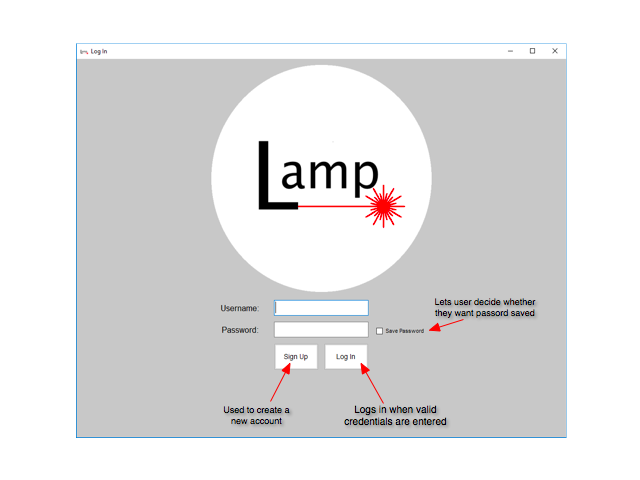
\includegraphics[width=0.7\textwidth]{screen/login.png}
\caption{The Login Screen was created with simplicity in mind, and so the only things on the screen upon the start-up are the logo and the textboxes that you login with. The form uses a light grey background colour, which is consistent throughout all the forms of the program.}
\end{figure}

\subsection{Sign Up}
% sign up screen
\begin{figure}[H]
	\centering
	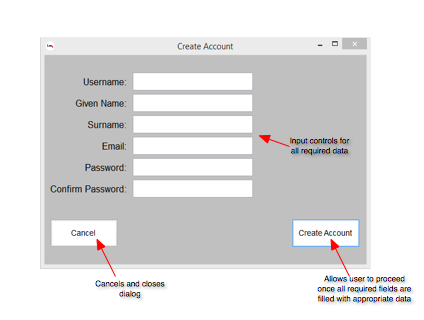
\includegraphics[width=0.7\textwidth]{screen/signup.png}
	\caption{This screen contains only text boxes and labels to guide the user as to how to sign up and create an account.}
\end{figure}

\subsection{Home Screen}
% home screen
\begin{figure}[H]
	\centering
	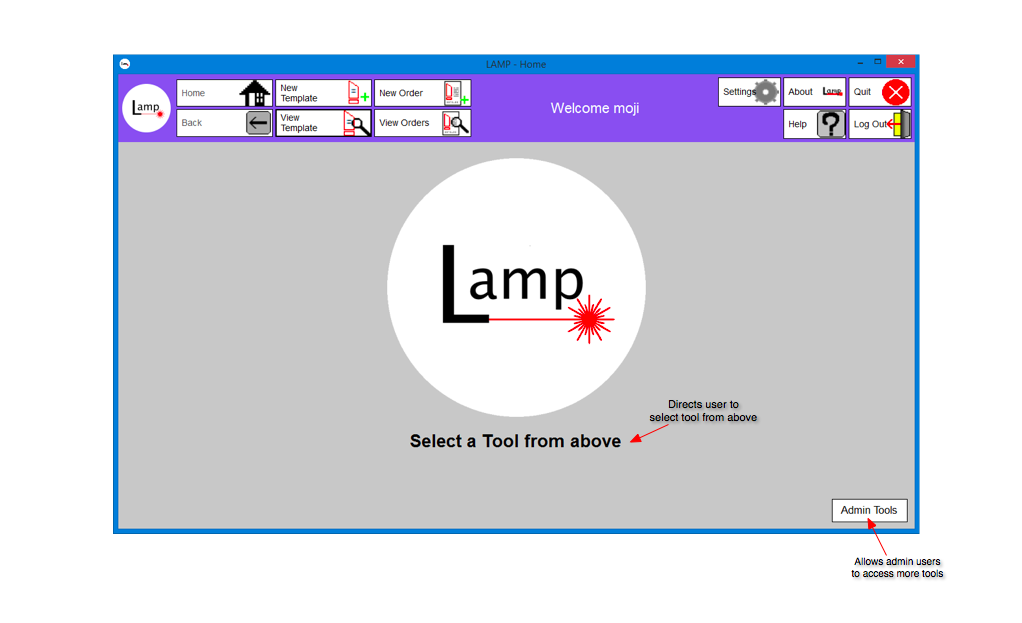
\includegraphics[width=0.7\textwidth]{screen/home.png}
	\caption{This screen has a toolbar which is also consistent throughout the program. It also contains links to the other forms }
\end{figure}

\subsection{Create New Template}
% Design screen
\begin{figure}[H]
	\centering
	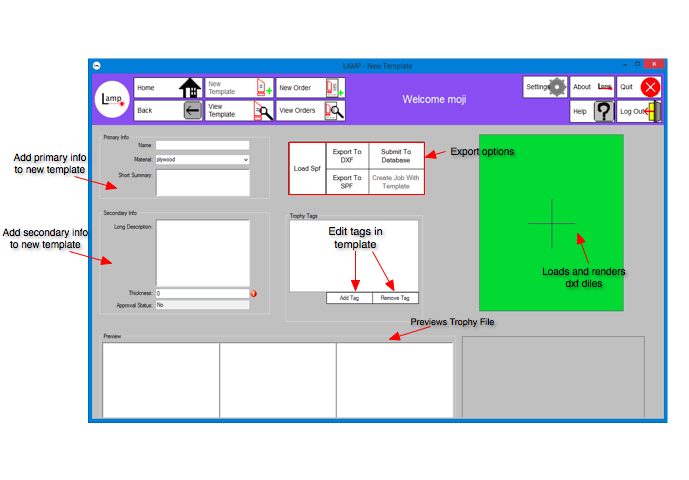
\includegraphics[width=0.7\textwidth]{screen/newtemplate.png}
	\caption{This screen allows users to create new templates, which can be stored in a database or exported to a .spf file}
\end{figure}

\subsection{View Templates}
% Design screen
\begin{figure}[H]
	\centering
	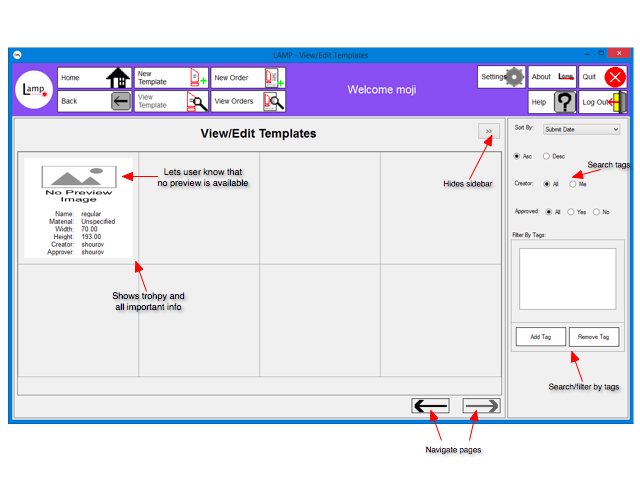
\includegraphics[width=0.7\textwidth]{screen/templateviewer.png}
	\caption{This screen allows users to search and sort the database for templates}
\end{figure}

\subsection{Create Job (1/2)}
\begin{figure}[H]
	\centering
	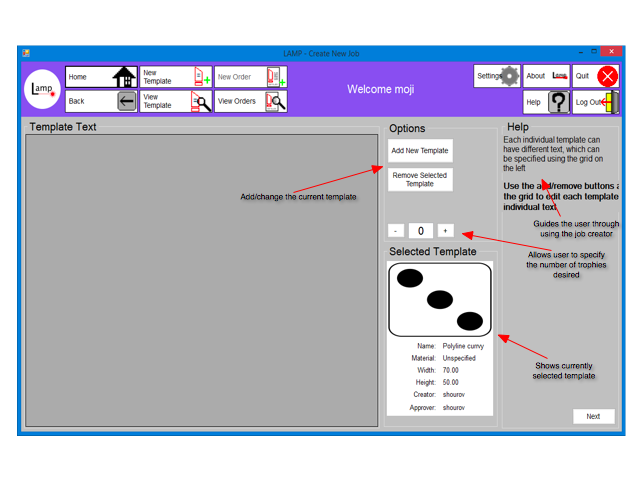
\includegraphics[width=0.7\textwidth]{screen/createjob.png}
	\caption{Once a template is selected, a user can choose the number of templates required. The grid allows easy manipulation of text that will be placed on the template in the next step}
\end{figure}

\subsection{Create Job (2/2)}
\begin{figure}[H]
	\centering
	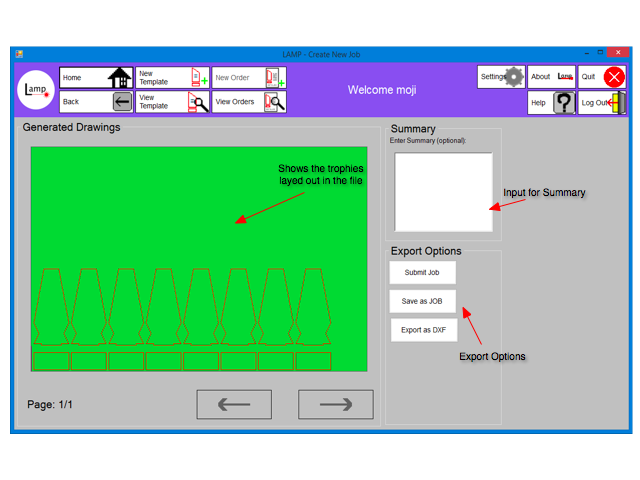
\includegraphics[width=0.7\textwidth]{screen/submitjob.png}
	\caption{The output and number of sheets required are shown on this screen, as long as options to export the job to the database or as a local file}
\end{figure}

\subsection{View Orders}
\begin{figure}[H]
	\centering
	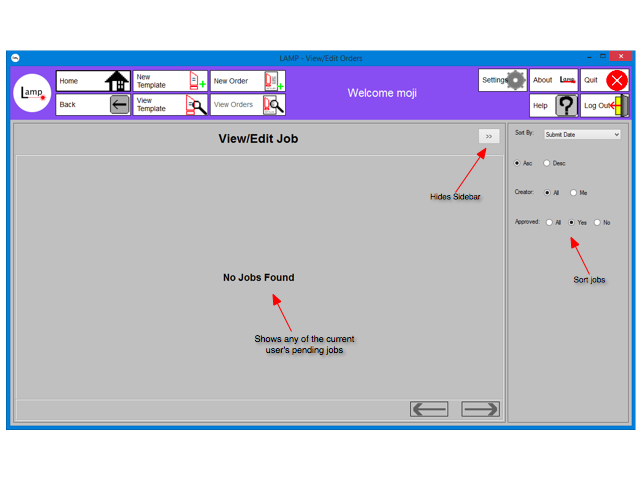
\includegraphics[width=0.7\textwidth]{screen/vieworders.png}
	\caption{Allows user to view the currently available orders}
\end{figure}



\subsection{Dialogs}
\begin{figure}[H]
	\centering
	\subsubsection{Help}
	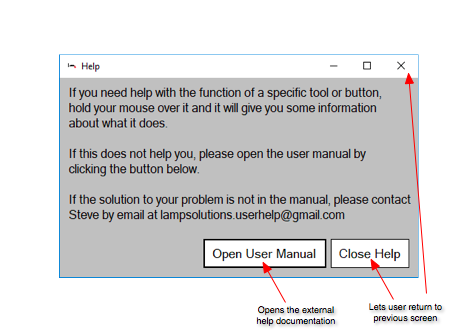
\includegraphics[width=0.5\textwidth]{screen/help.png}
	\caption{The help dialog informs the user how to use tooltips  and provides a link to the user manual}
\end{figure}
\begin{figure}[H]
	\centering
	\subsubsection{About}
	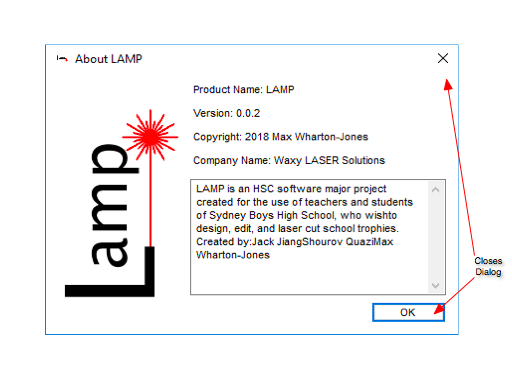
\includegraphics[width=0.5\textwidth]{screen/about.png}
	\caption{The about dialog provides information about the program along with relevant copyright and licensing terms}
\end{figure}

\begin{figure}[H]
	\centering
	\subsubsection{Logout}
	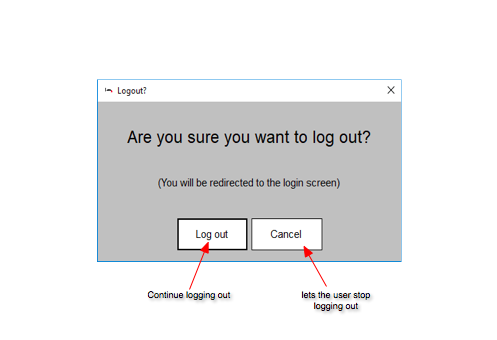
\includegraphics[width=0.5\textwidth]{screen/logout.png}
	\caption{This logout box provides feedback to the user when the logout button is pressed}
\end{figure}



\chapter{Testing and Evaluating the Solution}
\section{Test Data}
\subsection{Login}

\begin{longtable}{|p{3cm}|p{3cm}|p{3cm}|p{3cm}|p{3cm}|}
	\hline
	\rowcolor{gray!50}
	\textbf{Username} & \textbf{Password} & \textbf{Save Details} & \textbf{Expected Results} & \textbf{Reason}\\ \hline
	Valid Guest Username - “guest0” & Corresponding Password & Yes & Guest logs in and credentials are saved for login next time. Access level 0 & Valid credentials were entered and the login details were saved \\ \hline
	
	Valid User Username - “user1” & Corresponding Password & No & Student Logs in and credentials are not saved for login next time. Access level 1 &  Valid credentials were entered and the login details were not told to be saved \\ \hline
	
Valid Teacher Username - “teacher1” & 	Corresponding Password & Yes & Student logs in and credentials are saved for login next time. Access level 2 & Valid credentials were entered and the login details were saved \\ \hline

Valid Admin Username & Corresponding Password & No & Admin Logs in and credentials are saved for login next time. Access level 3 & Valid credentials were entered and the login details were not told to be saved \\ \hline

Valid Username & Invalid Password & No & Invalid Credentials Error popup & Invalid password was given \\ \hline

Invalid Username “-qeirj92-fikfl” & Invalid Password & No & Invalid Credentials. Error popup & Invalid username was given \\ \hline
	
\end{longtable}

\subsection{View Template / Add Template}
\begin{longtable}{|p{3cm}|p{3cm}|p{3cm}|p{3cm}|p{3cm}|}
	\hline
	\rowcolor{gray!50}
	\textbf{Selected Template} & \textbf{Field} & \textbf{Input} & \textbf{Expected Results} & \textbf{Reason}\\ \hline
	
	Template1 & Name & Template2 & Confirmation box followed by confirmation of change & User has submitted a valid change to the template, hence updating the template in the database \\ \hline
	
	Template1 & Name & "" & Error message indicating invalid input as well as visual indication of the offending field & User has submitted an invalid change to the template, hence the program will not allow submission until changes are validated \\ \hline
	
	Template1  & Thickness & 2 & Confirmation box followed by confirmation of change & User has submitted a valid change to the template, hence updating the template in the database \\ \hline
	
	Template1 & Thickness & two &Error message indicating invalid input as well as visual indication of the offending field & User has submitted an invalid change to the template, hence the program will not allow submission until changes are validated \\ \hline
\end{longtable}


\subsection{View Template / Add Tags  AND NewTemplate / Add Tags}
\begin{longtable}{|p{3cm}|p{6cm}|p{6cm}|}
	\hline
	\rowcolor{gray!50}
	\textbf{Input} &  \textbf{Expected Results} & \textbf{Reason} \\ \hline
	
	Wood & Tag is added to the template and is seen under the tags table & Tag is valid and is added to the template file \\ \hline
	
	"" & Tag is not added to the template and an error message is supplied & Tag is invalid and hence will not be added to the template \\ \hline
\end{longtable}

\subsection{New Order}
\begin{longtable}{|p{3cm}|p{3cm}|p{4.5cm}|p{4.5cm}|}
	\hline
	\rowcolor{gray!50}
	\textbf{Field} & \textbf{Input} &  \textbf{Expected Results} & \textbf{Reason} \\ \hline
	
	Add Tags & Grid Viewer shows all templates with a tag including “Wood” in them & Input tag is valid and hence the database shown is limited to the input tag \\ \hline
	
	Add Tags & "" & Error message is shown indicating tag cannot be empty & Input tag is invalid and hence feedback is given to the user to validate the tag \\ \hline
	
\end{longtable}

\subsection{New Job}
\begin{longtable}{|p{3cm}|p{3cm}|p{4.5cm}|p{4.5cm}|}
	\hline
	\rowcolor{gray!50}
	\textbf{Field} & \textbf{Input} &  \textbf{Expected Results} & \textbf{Reason} \\ \hline
	
	Number Of Jobs & 3 & Number is updated to indicate the number of jobs & Input is valid and hence the number of drawings generated in the job is increased to the input amount \\ \hline
	
	Number Of Jobs & 100,000 & Number is updated to indicate the number of jobs & Input is valid and hence the number of drawings generated in the job is increased to the input amount \\ \hline
	
	Number Of Jobs & three & Visual indicator of invalid input & Input is invalid and hence a visual indication is generated to indicate the corrupting field. \\ \hline
	
\end{longtable}

\subsection{New Job Boundaries (Optional)}
\begin{longtable}{|p{3cm}|p{3cm}|p{4.5cm}|p{4.5cm}|}
	\hline
	\rowcolor{gray!50}
	\textbf{Dynamic Text} & \textbf{Input} &  \textbf{Expected Results} & \textbf{Reason} \\ \hline
	
	Name & John Doe &Dynamic Text is seen on table & Dynamic Text has been added by the user for the given job \\ \hline
	
\end{longtable}

\subsection{Add New User / Edit User}
\begin{longtable}{|p{3cm}|p{3cm}|p{4.5cm}|p{4.5cm}|}
	\hline
	\rowcolor{gray!50}
	\textbf{Field} & \textbf{Input} &  \textbf{Expected Results} & \textbf{Reason} \\ \hline
	
	Username & John Doe &	Field is updated with input &	Input is valid and is added to the user file \\ \hline
	Username &	“” &	A red marker is generated to indicate an error.	& Input is invalid and a visual error is generated to indicate the offending field \\ \hline
	Password & password123 & Field is updated with input & Input is valid and is added to the user file \\ \hline
	Password & “” & A red marker is generated to indicate an error. & Input is invalid and a visual error is generated to indicate the offending field \\ \hline
	Name & John	& Field is updated with input &Input is valid and is added to the user file \\ \hline
	Name & “” & A red marker is generated to indicate an error. & Input is invalid and a visual error is generated to indicate the offending field \\ \hline
	Email &johndoe@email.com & Field is updated with input & Input is valid and is added to the user file \\ \hline
	Email & “” & A red marker is generated to indicate an error. & Input is invalid and a visual error is generated to indicate the offending field \\ \hline
	Email & johndoeemail & A red marker is generated to indicate an error. & Input is invalid and a visual error is generated to indicate the offending field \\ \hline
	Email & johndoe@email & A red marker is generated to indicate an error. & Input is invalid and a visual error is generated to indicate the offending field \\ \hline
	
\end{longtable}

\subsection{System Level Testing}
\subsubsection{Hardware}
Both the Application and the Server were tested on three different Windows Machines: A Windows 10 PC (i5 6600, 16gb RAM), Windows 7 Laptop (i3, 4gb RAM) and on a School Machine (Pentium, 8gb RAM).
\subsubsection{Software}
L.A.M.P was tested with various different .net framework versions(.net 4.5-7), and with a variety of external CAD programs.
\subsubsection{Data}
The database was loaded with different amounts of data:\\
\textbf{Templates}
\begin{longtable}{|p{5cm}|p{5cm}|}
	\hline
	\rowcolor{gray!50}
	\textbf{Files} & \textbf{Database Size}   \\ \hline

	10 templates & 6 mb  \\ \hline
	20 templates & 9 mb  \\ \hline
	30 templates & 10 mb  \\ \hline
	40 templates & 12 mb  \\ \hline
	100 templates & 18 mb  \\ \hline

\end{longtable}
Due to SQLITE's automatic compression of dxf files, aided by the similar structure of said files, we found that storing many templates in the database was not a problem

\textbf{Jobs}

\begin{longtable}{|p{5cm}|p{5cm}|}
	\hline
	\rowcolor{gray!50}
	\textbf{Files} & \textbf{Database Size}   \\ \hline
	
	10 jobs & 14 mb  \\ \hline
	20 jobs & 20 mb  \\ \hline
	30 jobs & 35 mb  \\ \hline
	40 jobs & 40 mb  \\ \hline
	100 jobs & 80 mb  \\ \hline
	
\end{longtable}

Similarly, we found that SQLITE's compression helped reduce the storage space of jobs. However, since jobs are larger files, it required more memory that with an equal number of templates.


Despite the large amounts of data stored by LAMP, the database never grew unmanageably big, due to automatic compression. A database containing both 100 jobs and templates will require approximately 100 megabytes of storage.

\subsubsection{Response Times}
We tested response times on two different machines, a developer machine (i5, 16gb RAM), and on the school computer (pentium, 8gb RAM), to the nearest 100 milliseconds (ms).
\begin{longtable}{|p{7cm}|p{3cm}|p{3cm}|}
	\hline
	\rowcolor{gray!50}
	\textbf{Task} & \textbf{Time for Developer Machine (ms)} &  \textbf{Time for School Machine (ms)}  \\ \hline
	Startup & 400 & 500  \\ \hline

	Insert Line into Drawing & $<$ 100 & $<$ 100  \\ \hline
	Insert Circle into Drawing & $<$ 100 & $<$ 100  \\ \hline
	Insert Static Text into Drawing & $<$ 100 & $<$ 100  \\ \hline
	Insert Dynamic Text into Drawing & $<$ 100 & $<$ 100  \\ \hline
	
	Save SPF (varies due to file size differences) & 500-1200 & 600-2000  \\ \hline
	Save DXF (varies due to file size differences) & 200-500 & 300-700 \\ \hline
	
	Get Template List & 300-1800 & 300-1800  \\ \hline
	Get Job List & 400-2000 & 800-2000  \\ \hline

	Submit/Edit Template & 500-1300 & 500-1300 \\ \hline
	Submit/Edit Job & 600-1500 & 600-1600  \\ \hline
	
	Delete Template & 200-400 & 200-400 \\ \hline
	Delete Job & 200-400 & 200-400  \\ \hline
\end{longtable}

These results were collected using Passmark's AppTimer, and with visual studio's Benchmark Test Explorer. 
There was only a small difference in response time between the school and developer machine, enough though the developer machine had almost twice the computing power. This is likely due to the bottleneck being the hard drive and network speed, since there is little heavy computation required. For tasks longer than a second, a loading screen will need to be provided in order to provide feedback for the user. 

\subsection{Beta Testing}
Our program was beta tested by two members of our software class and by Ms. Dam
\subsubsection{Version 0.4}
\textbf{Tester: Brian.} \\
Brian remarked that the program’s interface did not flow correctly, often requiring the use of the X button in the window bar in order to return to a previous form. This resulted in a non-optimal user experience. One form, DESIGNER FORM was found to be almost unusable due to lack of help and the complexity of form (holding several designing tools that were non uniformly spaced), and needs to be redesigned. However, he was ultimately able to create basic templates after a short learning period using an external CAD program instead of LAMP’s inbuilt open. From this, we learnt that the user interface was lacking and needed judicious use of both color and icons to improve its usability. Beta testing also revealed several bugs that caused LAMP to crash, including an error that caused the program to crash when the back button was pressed with no previous form.


\subsubsection{Version 0.6}
\textbf{Tester: Vincent} \\
This version of the program was more polished, with Vincent able to create templates from a provided dxf file, although a detailed walkthrough was required by LAMP employees. However, the program still contained several bugs that caused crashes that needed to be fixed, for example, loading an invalid or incorrect file caused the program to terminate. We also observed that the use of icons allowed Vincent to better navigate the program.

\subsubsection{Version 1.0.2}
\textbf{Tester: Ms Dam} \\
With the program entering ‘stable’ release, Ms Dam marked our program. However, a few bugs still existed.
An incorrect compiler resulted in integer overflow, which resulted in program termination. Ms Dam also noticed that the dynamic text interface
was hard to use by a new user, which could be improved in on future iterations. However, the core functionality of the program: generating
templates which could be submitted as jobs to the IA staff was successfully used, although many small patches could be applied to greatly
improve the experience.


\section{Evaluation of the Final Solution}
\begin{longtable}{|p{4cm}|p{2cm}|p{8cm}|}
	
	\hline
	\rowcolor{gray!50}
	\textbf{Needs} & \textbf{Objectives} & \textbf{Evaluation of Objective} \\ \hline
	
	Must store $>50$ different records & 
	Yes &
	The program can store well over 50 templates, but as more templates enter the database, the loading and searching/sorting times will slow slightly. 
	\\ \hline
	
	Ability to store many types of users. e.g. clients, users. &
	Yes &
	The program currently assigns an access level to each user based on their position at the school. 0: guest, 1: student, 2: teacher, 3: admin, 4: LAMP employees/developers 
	\\ \hline
	
	Store fonts and different shapes &
	Yes &
	The program can write and read different fonts and create different shapes in the designer.
	\\ \hline
	
	A drag-and-drop interface supporting:
	\begin{itemize}
		\itemsep0em
		\item text with different fonts
		\item circles
		\item rectangles
		\item lines
	\end{itemize} &
	Yes &
	The trophy designer can both take a trophy file and loads it into LAMP, as well as edit the design or create a new one using lines, circles and other tools. 
	\\ \hline
	
	Program must indicate the material and settings to use on the laser cutter, OR setting these values automatically before a job. &
	Partially &
	Using the summary section of the job, the user can specify what settings will need to be applied, but this would be difficult for an average user to do as the settings are quite specific. 
	\\ \hline
	
	The program must be efficient in the usage and process of its materials. For example, when engraving school trophies for Sydney Boys High School & 
	Yes &
	The program is optimized so that a single job will have the maximum level of efficiency by effectively grouping trophies together using a specialized algorithm, therefore minimizing waste. \newline The jobs are scanned to ensure laser cutting integrity is maintained, this is done by analysing line types and ensuring no erroneous lines or shapes are present in the file. This will increase the speed of laser cutting. \\ \hline
	
	The program must be optimised such at LEAST 8 trophies can be cut per hour. &
	Yes &
	Due to the time saving methods listed above, the trophies can be printed more efficiently, saving time and increasing cuts per hour.
	\\ \hline
	
	Program must assist the user in aligning the job in the laser cutter. Previously this was done manually with callipers. &
	Yes &
	Since the program produces a file with multiple trophies lain out in one file, the alignment of trophies is done automatically, thus the operator of the laser cutter will only need to insert a large sheet of material, and press cut.
	\\ \hline
	
	To increase efficiency of the cutter:
	\begin{itemize}
		\itemsep0em
		\item Reduce Raster lines
		\item Increase Vector Lines
		\item No double lines
		\item Vector-based fonts
	\end{itemize} &
	Partially &
	The program filters out some duplicated lines and removes invalid lines. However, improvements can be made in order to further increase efficiency.
	\\ \hline
	
	Current GUI has many issues, that must be rectified in the solution
	\begin{itemize}
		\itemsep0em
		\item Hard to navigate
		\item Limited usage
		\item No tutorial
		\item No colour
		\item Some functions don’t work such as key bindings
		\item Hard to line up
	\end{itemize} & 
	Yes &
	The GUI has been made more intuitive with the inclusion of on-screen prompts and tooltips, while maintaining a clean, material look to minimize clutter.\newline The capabilities of the program have been greatly increased, with more tools and functions for the user to use. The program now includes a dedicated help document to guide the user through all aspects of the application.
	\\ \hline
	Ability to export/import files compatible with illustrator AND/OR AutoCAD or other popular cad programs &
	Yes &
	Both illustrator and AutoCAD files can be imported into the designer, or straight into the database for personal or public use.
	\\ \hline
	
	Ability to attach a number of tags to each template, which can be filtered by the user
	Sort/Search by:
		\begin{itemize}
		\itemsep0em
		\item Template name
		\item Template creator
		\item Date created/Approved
		\item Item ID
		\item Template material
	\end{itemize} & 
	Yes &
	When uploading a trophy to the database, or editing the database, tags can be added or removed from the database files. The tags are used by the searching and sorting function of the database, allowing users to filter out unwanted specifications such as acrylic or wood.
	\\ \hline
	
	Three modes: 
		\begin{itemize}
		\itemsep0em
		\item Cut trophy mode, someone manually lines blank trophies up as shown by the program, and a pattern is cut onto it
		\item Cut Plaque mode, a sheet of material is cut using the laser cutter into smaller plaques
		\item Net mode, a net is generated dynamically based on constraints given by the user: e.g. a box can be generated from length, height, width and whether it is closed or open
	\end{itemize} & 
	Yes &
	LAMP can be used to not only create trophies and plaques, but to create any file that a user would like to laser cut.\newline
	We have made the program more generic by not forcing the user to switch between different modes to cut different things.
	\\ \hline
	3 levels of access, with each level having all the permissions of the levels below 
		\begin{itemize}
		\itemsep0em
		\item Student (Lowest): can submit templates to be approved then used by teachers/administrators
		\item Teachers: can also submit jobs to administrators for approval, who run the laser cutter. Can also approve templates.
		\item Administrators: have all permissions, can view all information and approve all jobs/templates, to be cut by the laser cutter.
	\end{itemize} & 
	Yes &
The access levels have been slightly changed with an inclusion of a guest level (level 0), then all levels proceed as originally planned, with the higher levels possessing all features of the level(s) below.\newline Administrators have access to the admin home, which is used to approve or deny jobs and approve additions to the database. \\ \hline
	A process that reads in an Illustrator file and
		\begin{itemize}
		\itemsep0em
		\item Reads all linetypes in the file
		\item Compiles linetypes in numerical data
		\item Quantitatively assesses linetype data
		\item Provides estimate on print time
		\item Displays linetype data in readable format
	\end{itemize} & 
	No &
	This has now been replaced with a newer method, spf files, which contain the design, as well as tags. \newline
	Due to the validation of the files, the print time estimation supplied by the laser cutter print driver is more accurate, hence the need for developing our own print time calculator is non-existent. \\ \hline
\end{longtable}

\subsubsection{Conclusion}
The quality of the solution could be improved by making the UI less cluttered, containing more intuitive controls and layouts, as will as more tooltips and prompts. Many quality of life improvements could also be made to the solution including:
	
	\begin{itemize}
	\itemsep0em
	\item Not resizing a form when a new function is being used and a new form is opened
	\item Forms appearing in the same location as the previous form
	\item More tooltips
	\item Updated help document
	\item Back button working with multiple screens on the same form
\end{itemize} 
	
	
	
	
	
	
	
\end{document}


